% !TEX program = xelatex
% 全国大学生嵌入式芯片与系统设计竞赛 - 应用赛道作品设计报告
% 注意：全文不写学校、指导教师、个人账号、私有 IP 或 API Key。
\documentclass[a4paper,12pt]{ctexart}

\usepackage[a4paper,top=2.4cm,bottom=2.2cm,left=2.3cm,right=2.3cm]{geometry}
\usepackage{setspace}\onehalfspacing
\usepackage{amsmath,amssymb}
\usepackage{graphicx}\graphicspath{{figs/}}
\usepackage{booktabs,longtable,array,multirow,makecell}
\usepackage{float}
\usepackage[section]{placeins}
\usepackage{etoolbox}
\AtBeginDocument{\preto\subsection{\FloatBarrier}}
\usepackage{xcolor}
\usepackage{enumitem}\setlist{nosep,leftmargin=1.7em}
\usepackage{tcolorbox}\tcbuselibrary{skins,breakable}
\usepackage{fancyhdr}
\usepackage{titlesec}
\usepackage[hidelinks]{hyperref}
\urlstyle{same}
\usepackage[font=small,labelfont=bf,labelsep=period]{caption}
\usepackage{subcaption}
\usepackage{indentfirst}

\definecolor{navy}{HTML}{1F3B57}
\definecolor{accent}{HTML}{2E7DF2}
\definecolor{teal}{HTML}{0FA9A4}
\definecolor{amber}{HTML}{F3A51B}
\definecolor{orange}{HTML}{F2682A}
\definecolor{good}{HTML}{17A65A}
\definecolor{red}{HTML}{EF4444}
\definecolor{panelbg}{HTML}{F4F7FB}
\definecolor{line}{HTML}{DCE5EF}

\titleformat{\section}{\Large\bfseries}{\thesection}{0.6em}{}
\titleformat{\subsection}{\large\bfseries}{\thesubsection}{0.6em}{}
\titleformat{\subsubsection}{\normalsize\bfseries}{\thesubsubsection}{0.6em}{}
\titlespacing*{\section}{0pt}{1.4ex plus 1ex}{0.8ex}
\titlespacing*{\subsection}{0pt}{1.1ex plus .5ex}{0.55ex}
\setlength{\headheight}{14.5pt}

\pagestyle{fancy}\fancyhf{}
\lhead{\small 双 RDK X5 异构协同材料合成 AI 与多机具身实验助理机器人}
\rhead{\small 作品设计报告}
\cfoot{\small\thepage}
\renewcommand{\headrulewidth}{0.4pt}

\newcommand{\kw}[1]{\textbf{#1}}
\newtcolorbox{keybox}[1][]{enhanced,colback=panelbg,colframe=navy,
  boxrule=0.8pt,arc=2pt,left=7pt,right=7pt,top=5pt,bottom=5pt,breakable,#1}
\newtcolorbox{warnbox}[1][]{enhanced,colback=red!4,colframe=red,
  boxrule=0.8pt,arc=2pt,left=7pt,right=7pt,top=5pt,bottom=5pt,breakable,#1}
\newtcolorbox{placeholderbox}[1][]{enhanced,colback=white,colframe=orange,
  boxrule=0.9pt,arc=2pt,left=7pt,right=7pt,top=8pt,bottom=8pt,breakable,#1}

\begin{document}

\thispagestyle{empty}
\vspace*{0.2em}
{\centering
{\LARGE\bfseries 基于双 RDK X5 异构协同的材料合成 AI 预测与多机具身实验助理机器人}\par
\vspace{0.5em}
{\large\bfseries ——AI 脑、具身脑、双机械臂工位与 STM32F407 执行层的材料实验闭环系统}\par
}
\vspace{1.1em}

\begin{center}
  \textbf{\large 摘 \quad 要}
\end{center}

本作品面向近红外荧光粉等功能材料研发中候选配方多、实验周期长、取放流程重复、XRD/PL 表征数据分散和失败经验难以回流的问题，构建了一套以 \kw{双 RDK X5 异构协同}为核心的嵌入式科研自动化系统。系统由实验室端 AI 脑、车载具身脑、双 myCobot 280-Pi 固定工位、STM32F407 下位机执行层和公网只读证据平台组成：AI 脑负责材料配方预测、XRD 与光谱分析、本地大模型推理和实验记录追溯；具身脑负责 LD14 激光雷达、Astra Pro 深度相机、里程计、SLAM 和 Lab-FSD shadow planner；固定工位负责粉末袋识别、夹取、转移与冗余接管；STM32F407 负责步进电机、电推杆、舵机和电磁铁的底层动作时序；公网平台负责状态孪生、演示剧场、OpenAPI、证据包和提交资产展示。

作品的核心不是单一网页、遥控车或机械臂展示，而是把“配方设计 $\rightarrow$ AI 预筛 $\rightarrow$ 具身取放 $\rightarrow$ XRD/PL 表征 $\rightarrow$ 失败回流”的材料实验链路拆分到多个嵌入式节点上，并通过本地推理、传感器融合和安全降级形成可展示、可追溯、可继续扩展的闭环。AI 脑侧采用总控 Dashboard 加 XRD 视觉、XRD 数值、PL 视觉、PL 数值四条表征分析线，结合 Shannon 半径规则、MACE/MatterSim/CHGNet 势能面缓存、Tanabe-Sugano 与 Huang-Rhys 光谱模型、失败规则库、Conformal 置信区间、本地 Qwen 系列与 DeepSeek 蒸馏模型，以及 Fly-MB/FlyHash 果蝇联想判决脑，输出候选配方风险、推荐烧结条件和可审计推理依据。具身脑侧将自动驾驶中的 BEV occupancy、未来占据和候选轨迹思想迁移到低速实验室机器人，形成 Lab-FSD 影子规划层；该层在线输出风险、候选轨迹和安全门控结果，但初赛阶段不直接发布底盘控制指令，由安全员保持执行权。

截至初赛提交前，系统已完成 AI 脑五服务线、4 个 CPU 本地模型、5 个 BPU swap-load 大模型槽、5 个轻量 BPU 感知模型、材料预测 evidence package、XRD/PL 表征分析、SLAM 占据栅格建图、Lab-FSD shadow 输出、arm01 视觉门控固定点取袋、F407 瓶子吸附/释放动作时序和公网证据平台部署。实测指标包括：Qwen2-0.5B 手写 Transformer 在 RDK X5 BPU 上完成 24 层链式推理，单次 forward 约 553 ms；Lab-FSD 影子规划毫秒级输出风险与轨迹；公网展示站提供 89 条 OpenAPI 路径；材料知识库侧完成 25228 段文献切片、67 行实测 PL 记录和多源规则/模型融合；机械臂工位完成末端相机视觉确认、AI 脑 station ok 判决、固定点取袋与落袋闭环。当前视频演示采用安全员接管底盘、末端执行安全降级和公网只读展示策略；后续补齐升降台限位、驱动隔离、地图质量优化和 Nav2 目标点后，可从 shadow mode 平滑升级到更完整的自主导航与实验执行闭环。

\vspace{0.8em}
\noindent\textbf{关键词：} RDK X5；嵌入式 AI；材料合成预测；XRD/PL 表征；具身实验机器人；Lab-FSD；SLAM；双机械臂；STM32F407

\vspace{0.4em}
\noindent\textbf{GitHub：} \url{https://github.com/Xiaomiju-x/xrd}

\newpage
\setcounter{page}{1}
\tableofcontents
\newpage

\section{第一部分 作品概述}

\subsection{功能与特点}
材料研发中的候选配方筛选通常需要多轮研磨、烧制、XRD、PL 光谱和人工判断。单个配方的真实实验耗时长、失败原因复杂，且视觉图像、数值谱图、配方记录和取放操作往往分散在不同设备上。本作品把这些环节统一到一个嵌入式系统中：先由 AI 脑完成候选配方预筛，再由具身脑和固定工位完成受控移动与取放，最后把表征结果回流到材料预测系统。

系统功能可以概括为六类：
\begin{enumerate}
  \item \kw{材料配方 AI 预筛：} 输入 host、掺杂离子和浓度后，输出发光波段、可行性等级、风险原因和推荐烧结条件。
  \item \kw{XRD/PL 四线分析：} 同时支持谱图图像和数值文件的检测、分类、解释和回流。
  \item \kw{移动感知与影子规划：} 车载 X5 运行 LiDAR、深度、里程计、SLAM 和 Lab-FSD shadow planner，输出风险和候选轨迹。
  \item \kw{固定工位取放：} 机械臂末端相机完成工位观察，AI 脑返回 \texttt{station\_ok} 后执行固定点取袋/落袋。
  \item \kw{下位机末端执行：} STM32F407 控制电推杆、舵机、电磁铁和升降机构，完成瓶子吸附、保持和释放的动作时序。
  \item \kw{公网只读证据平台：} 展示系统状态、演示剧场、全球对标、FSD 世界模型、机群和资产清单。
\end{enumerate}

\begin{figure}[H]
  \centering
  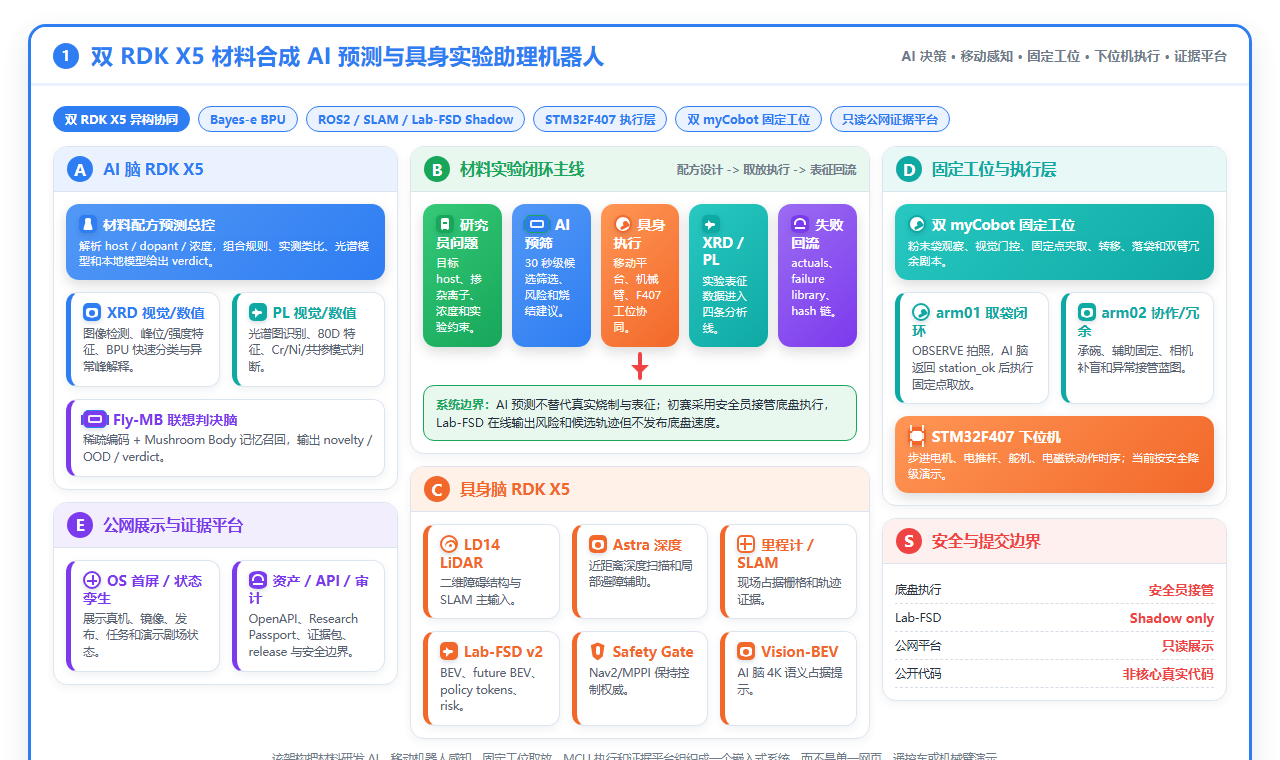
\includegraphics[width=\linewidth]{fig_xrd_architecture_html.png}
  \caption{双 RDK X5 材料合成 AI 预测与具身实验助理机器人总体架构。}
  \label{fig:xrd_arch}
\end{figure}

图~\ref{fig:xrd_arch} 展示了本作品的核心组织方式。AI 脑处理材料预测、四条表征线和 Fly-MB 联想判决；具身脑处理移动感知、SLAM 和 Lab-FSD shadow；固定工位和 F407 执行真实取放动作；公网平台仅承担只读展示和证据汇总。这种分层可以把复杂工程拆成可验证的子系统，避免把所有能力混在一个不可解释的“大模型演示”里。

\subsection{应用领域}
作品面向材料合成实验室，尤其适合近红外荧光粉、无机功能材料、陶瓷烧结和粉末体系的候选配方预筛与实验辅助。它的价值不是替代研究员，而是把高重复、长等待、强记录需求的实验环节转化为可计算、可执行、可回放的闭环任务。

该架构也可扩展到催化剂筛选、粉末冶金、陶瓷退火、半导体扩散炉监控和实验室危化品搬运等场景。只要实验流程同时具备“候选空间大、真实验证贵、动作重复、数据需要回流”这四类特征，就可以复用双边缘节点加固定工位的组织方式。

\subsection{主要技术特点}
本作品的技术特点可以概括为“边缘多模型、跨域异构、可验证执行和保密发布”。边缘多模型指 AI 脑在 RDK X5 上组合 BPU 轻量推理、CPU 本地模型、科学规则和实验知识库；跨域异构指材料预测、XRD/PL 表征、SLAM、机械臂和 F407 固件通过 API、ROS2 和串口状态机协同；可验证执行指所有真机能力均对应 evidence、日志、地图、状态矩阵或视频片段；保密发布指报告和开源包只公开接口、伪代码和非核心示例，不泄露模型权重、私有数据和危险控制入口。

\subsection{主要创新点}
\begin{enumerate}
  \item \kw{材料 AI 与具身实验的一体化闭环：} 将配方预筛、移动感知、固定工位取放、表征分析和失败回流放在同一系统叙事内。
  \item \kw{双 RDK X5 异构协同：} AI 脑承担科研推理和语义理解，具身脑承担传感器融合、SLAM 和安全影子规划。
  \item \kw{嵌入式多模型栈：} 在本地边缘平台上组合 BPU 轻量模型、BPU LLM slot、CPU 本地模型、科学规则和材料知识库。
  \item \kw{Lab-FSD shadow planner：} 将 BEV occupancy、未来占据和概率轨迹 token 映射到低速实验室机器人，并严格保持 observe-only 边界。
  \item \kw{视觉门控固定工位：} 机械臂不是盲目执行示教点，而是在 AI 脑视觉确认工位有效后执行固定点取放。
  \item \kw{证据链平台：} 把模型、API、演示剧场、发布记录、状态孪生和提交资产组织成可复核证据。
\end{enumerate}

\subsection{主要性能指标}
\begin{table}[H]
\centering
\caption{关键工程指标摘要。}
\begin{tabular}{p{4.0cm}p{3.1cm}p{7.0cm}}
\toprule
指标 & 当前结果 & 说明 \\
\midrule
AI 脑服务线 & 5 条 & 总控 Dashboard + XRD/PL 视觉与数值四条表征线 \\
CPU 本地模型 & 4 路 & 用于本地科研解释和断网降级 \\
BPU LLM slot & 5 个 & 用于 verdict probe 和工程展示，不宣传为实时长文本生成 \\
表征轻量模型 & 5 个能力位 & XRD/PL MLP、YOLO 和相关感知模型 \\
Qwen2 0.5B BPU forward & 约 553 ms & 手写 Transformer 分段后在 X5 BPU 上运行 \\
Lab-FSD BPU 异常观测 & 约 1.7 ms & 车载脑异常辅助模型工程观测值 \\
arm01 取袋闭环 & 已实测 & OBSERVE 拍照、AI 脑识别、\texttt{station\_ok} 后固定点取放 \\
公网接口规模 & 89 OpenAPI paths & 只读证据平台和状态展示接口 \\
\bottomrule
\end{tabular}
\end{table}

\begin{figure}[H]
  \centering
  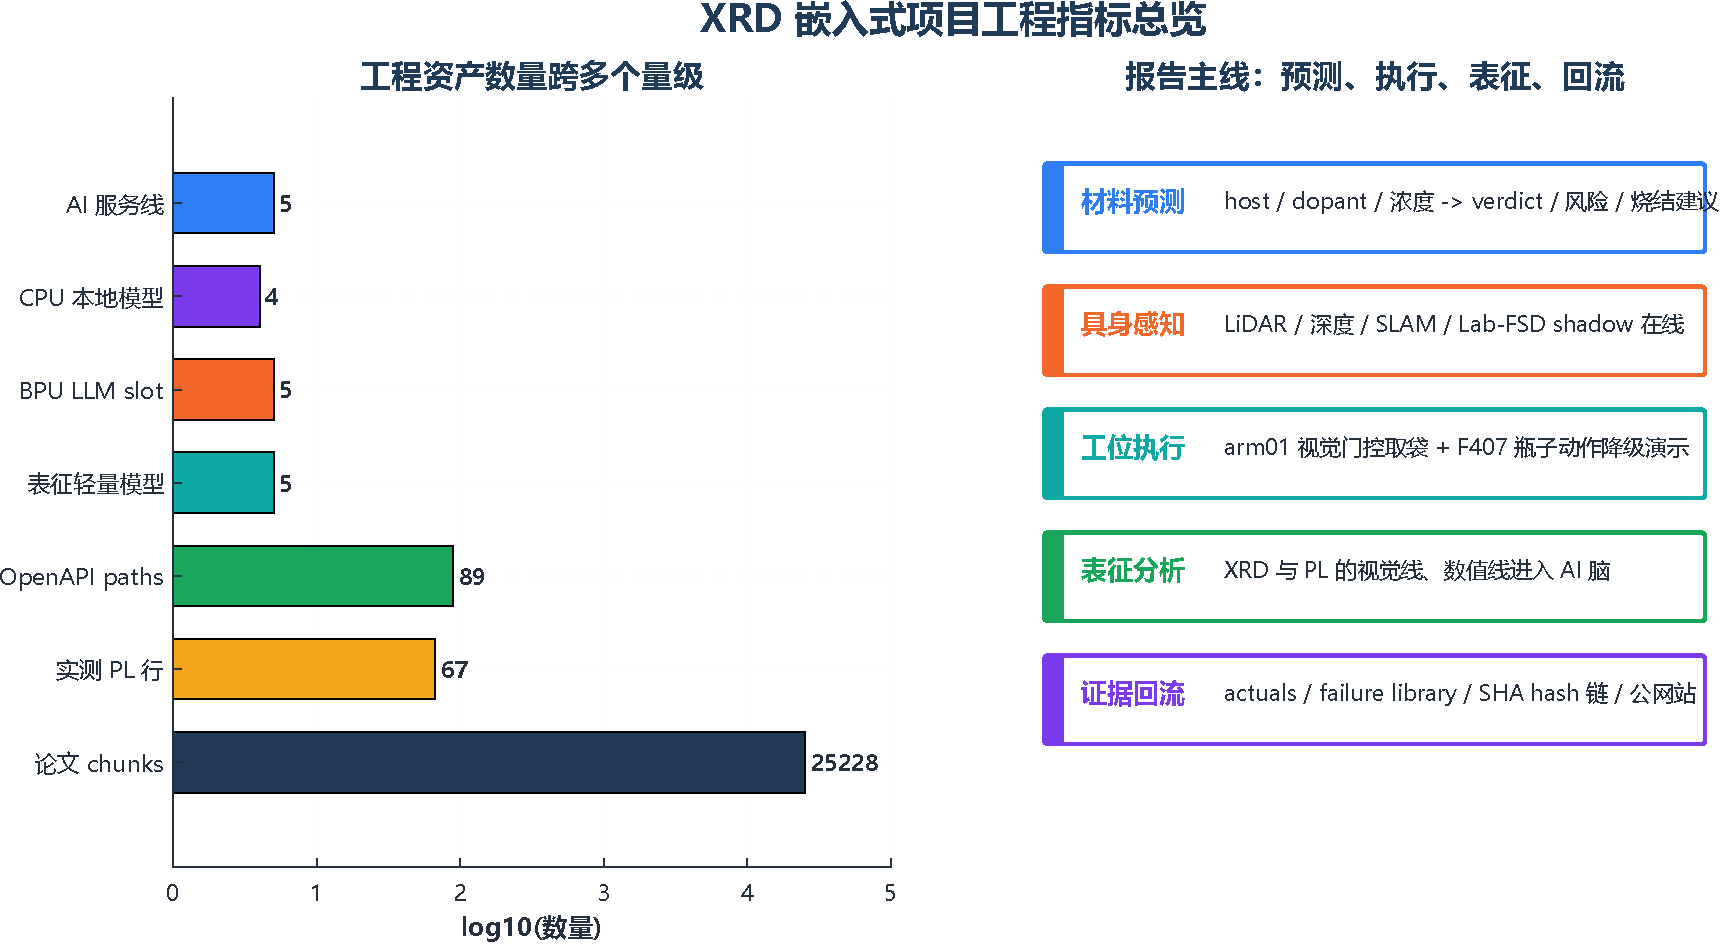
\includegraphics[width=0.96\linewidth]{fig_xrd_metrics.pdf}
  \caption{XRD 嵌入式项目工程指标总览。}
\end{figure}

\subsection{设计流程}
设计流程遵循“需求拆解 -> 系统分层 -> 单模块真机验证 -> 证据链汇总 -> 安全边界复核”的顺序。首先从材料研发周期长和实验取放重复的痛点出发，拆出 AI 预测、表征分析、移动感知、固定工位和底层执行五类任务；随后将任务分配给 AI 脑、具身脑、机械臂工位、F407 和公网证据平台；最后按已实测、shadow/降级和后续补齐三类状态整理初赛展示材料。

\section{第二部分 系统组成及功能说明（一）：需求分析与设计约束}

\subsection{材料实验痛点}
近红外荧光粉等材料体系通常存在候选配方多、物理机制复杂、真实烧制成本高的问题。研究员往往需要先提出一批候选，再逐个经历称量、研磨、烧制、XRD、PL 光谱和结果判断。若每轮要尝试 15-20 个候选，人工决策和实验等待会成为主要瓶颈。

本作品把需求拆成三个层次：第一层是 AI 预测，目的是在真实实验前快速排除高风险候选；第二层是具身执行，目的是让机器人承担可规范化的取放和转移动作；第三层是数据回流，目的是把实验结果变成下一轮预测的证据，而不是散落在截图、表格和人工记忆里。

\subsection{功能需求}
\begin{table}[H]
\centering
\caption{系统功能需求与对应实现。}
\begin{tabular}{p{3.5cm}p{5.4cm}p{5.8cm}}
\toprule
需求 & 设计实现 & 初赛状态 \\
\midrule
配方预筛 & AI 脑解析配方，调用物理模型、实测类比、本地模型和规则库 & 已跑通 \\
XRD/PL 分析 & 四条表征线分别处理视觉图像和数值谱图 & 已跑通 \\
移动感知 & 车载脑融合 LiDAR、深度、里程计并构建 SLAM 地图 & 已跑通 \\
影子规划 & Lab-FSD 输出 BEV、future BEV、policy token、risk 和 safety gate & 在线 shadow \\
末端执行 & F407 控制推杆、舵机、电磁铁和短行程升降动作 & 安全降级 \\
固定工位取放 & arm01 末端相机识别工位，AI 脑确认后固定点取袋 & 已实测 \\
证据展示 & 公网站展示状态、证据、API、发布和演示剧场 & 已部署 \\
\bottomrule
\end{tabular}
\end{table}

\subsection{嵌入式约束}
项目选择 RDK X5 的原因不是单纯追求模型参数规模，而是要在边缘设备上同时管理摄像头、BPU、CPU、本地服务、ROS2、传感器、机械执行和网络证据。设计中必须处理以下约束：
\begin{itemize}
  \item X5 不适合在线运行重型材料模拟或训练任务，MACE、MatterGen、LoRA 训练等放在 PC/云端预处理，X5 读取缓存和部署产物。
  \item BPU 的算子、CMA 和模型切段限制决定了 Transformer 只能以 slot / probe 方式工程展示，不能夸大为长文本实时生成。
  \item 移动底盘和升降台属于安全敏感执行器，初赛阶段必须采用安全员接管和硬件降级策略。
  \item 公网站点只能做状态展示和证据说明，不能下发底盘、机械臂、升降台、电磁铁等危险动作。
\end{itemize}

\begin{warnbox}
\textbf{安全原则：} 本作品报告中的“自主”“规划”“世界模型”均指算法在线运行和诊断输出。未完成全量安全验证的执行链路不写成无人值守闭环。
\end{warnbox}

\section{第二部分 系统组成及功能说明（二）：总体方案}

\subsection{端到端闭环}
系统的端到端闭环如图~\ref{fig:xrd_workflow} 所示。研究员输入材料目标后，AI 脑生成候选配方评审和推荐条件；具身脑负责移动感知、SLAM 和 shadow planning；固定工位负责粉末袋取放；F407 负责瓶子末端执行；XRD/PL 结果再回流到 AI 脑形成下一轮证据。

\begin{figure}[H]
  \centering
  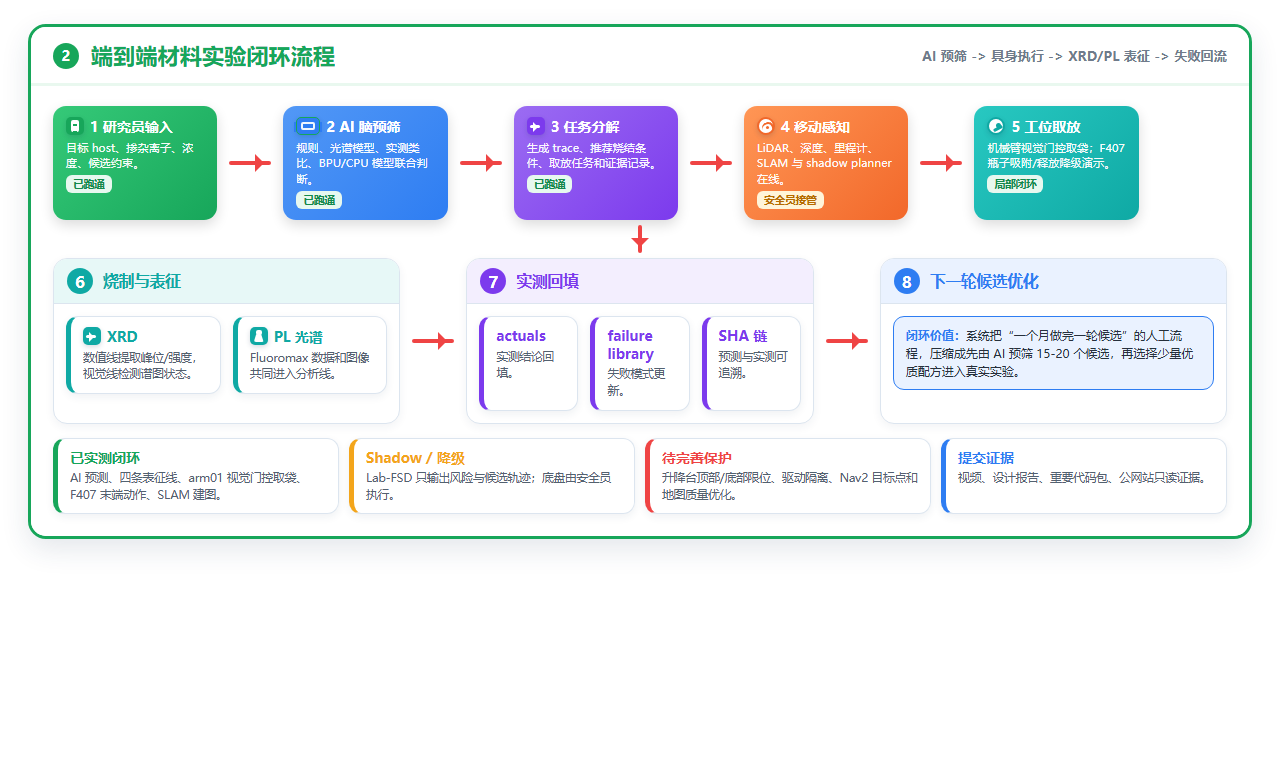
\includegraphics[width=\linewidth]{fig_xrd_workflow_html.png}
  \caption{端到端材料实验闭环流程。}
  \label{fig:xrd_workflow}
\end{figure}

图中绿色部分代表已有真机或服务证据，橙色代表初赛阶段采用安全降级或 shadow 模式，紫色代表后续扩展方向。这一分层是报告可信度的核心：有证据的写“已实测”，有算法在线但未接管执行的写“shadow/降级”，硬件保护未补齐的写“后续补齐”。

\subsection{硬件组成}
硬件系统由双 RDK X5、双 myCobot 280-Pi 固定工位、STM32F407 下位机、LD14 LiDAR、Astra 深度相机、IMX415 4K 相机、USB 相机、电推杆、舵机、步进电机和电磁铁组成。AI 脑和具身脑通过局域网和 API 协同，F407 通过串口接收动作指令，机械臂工位通过本臂控制器执行示教动作和状态回放。

\begin{figure}[H]
  \centering
  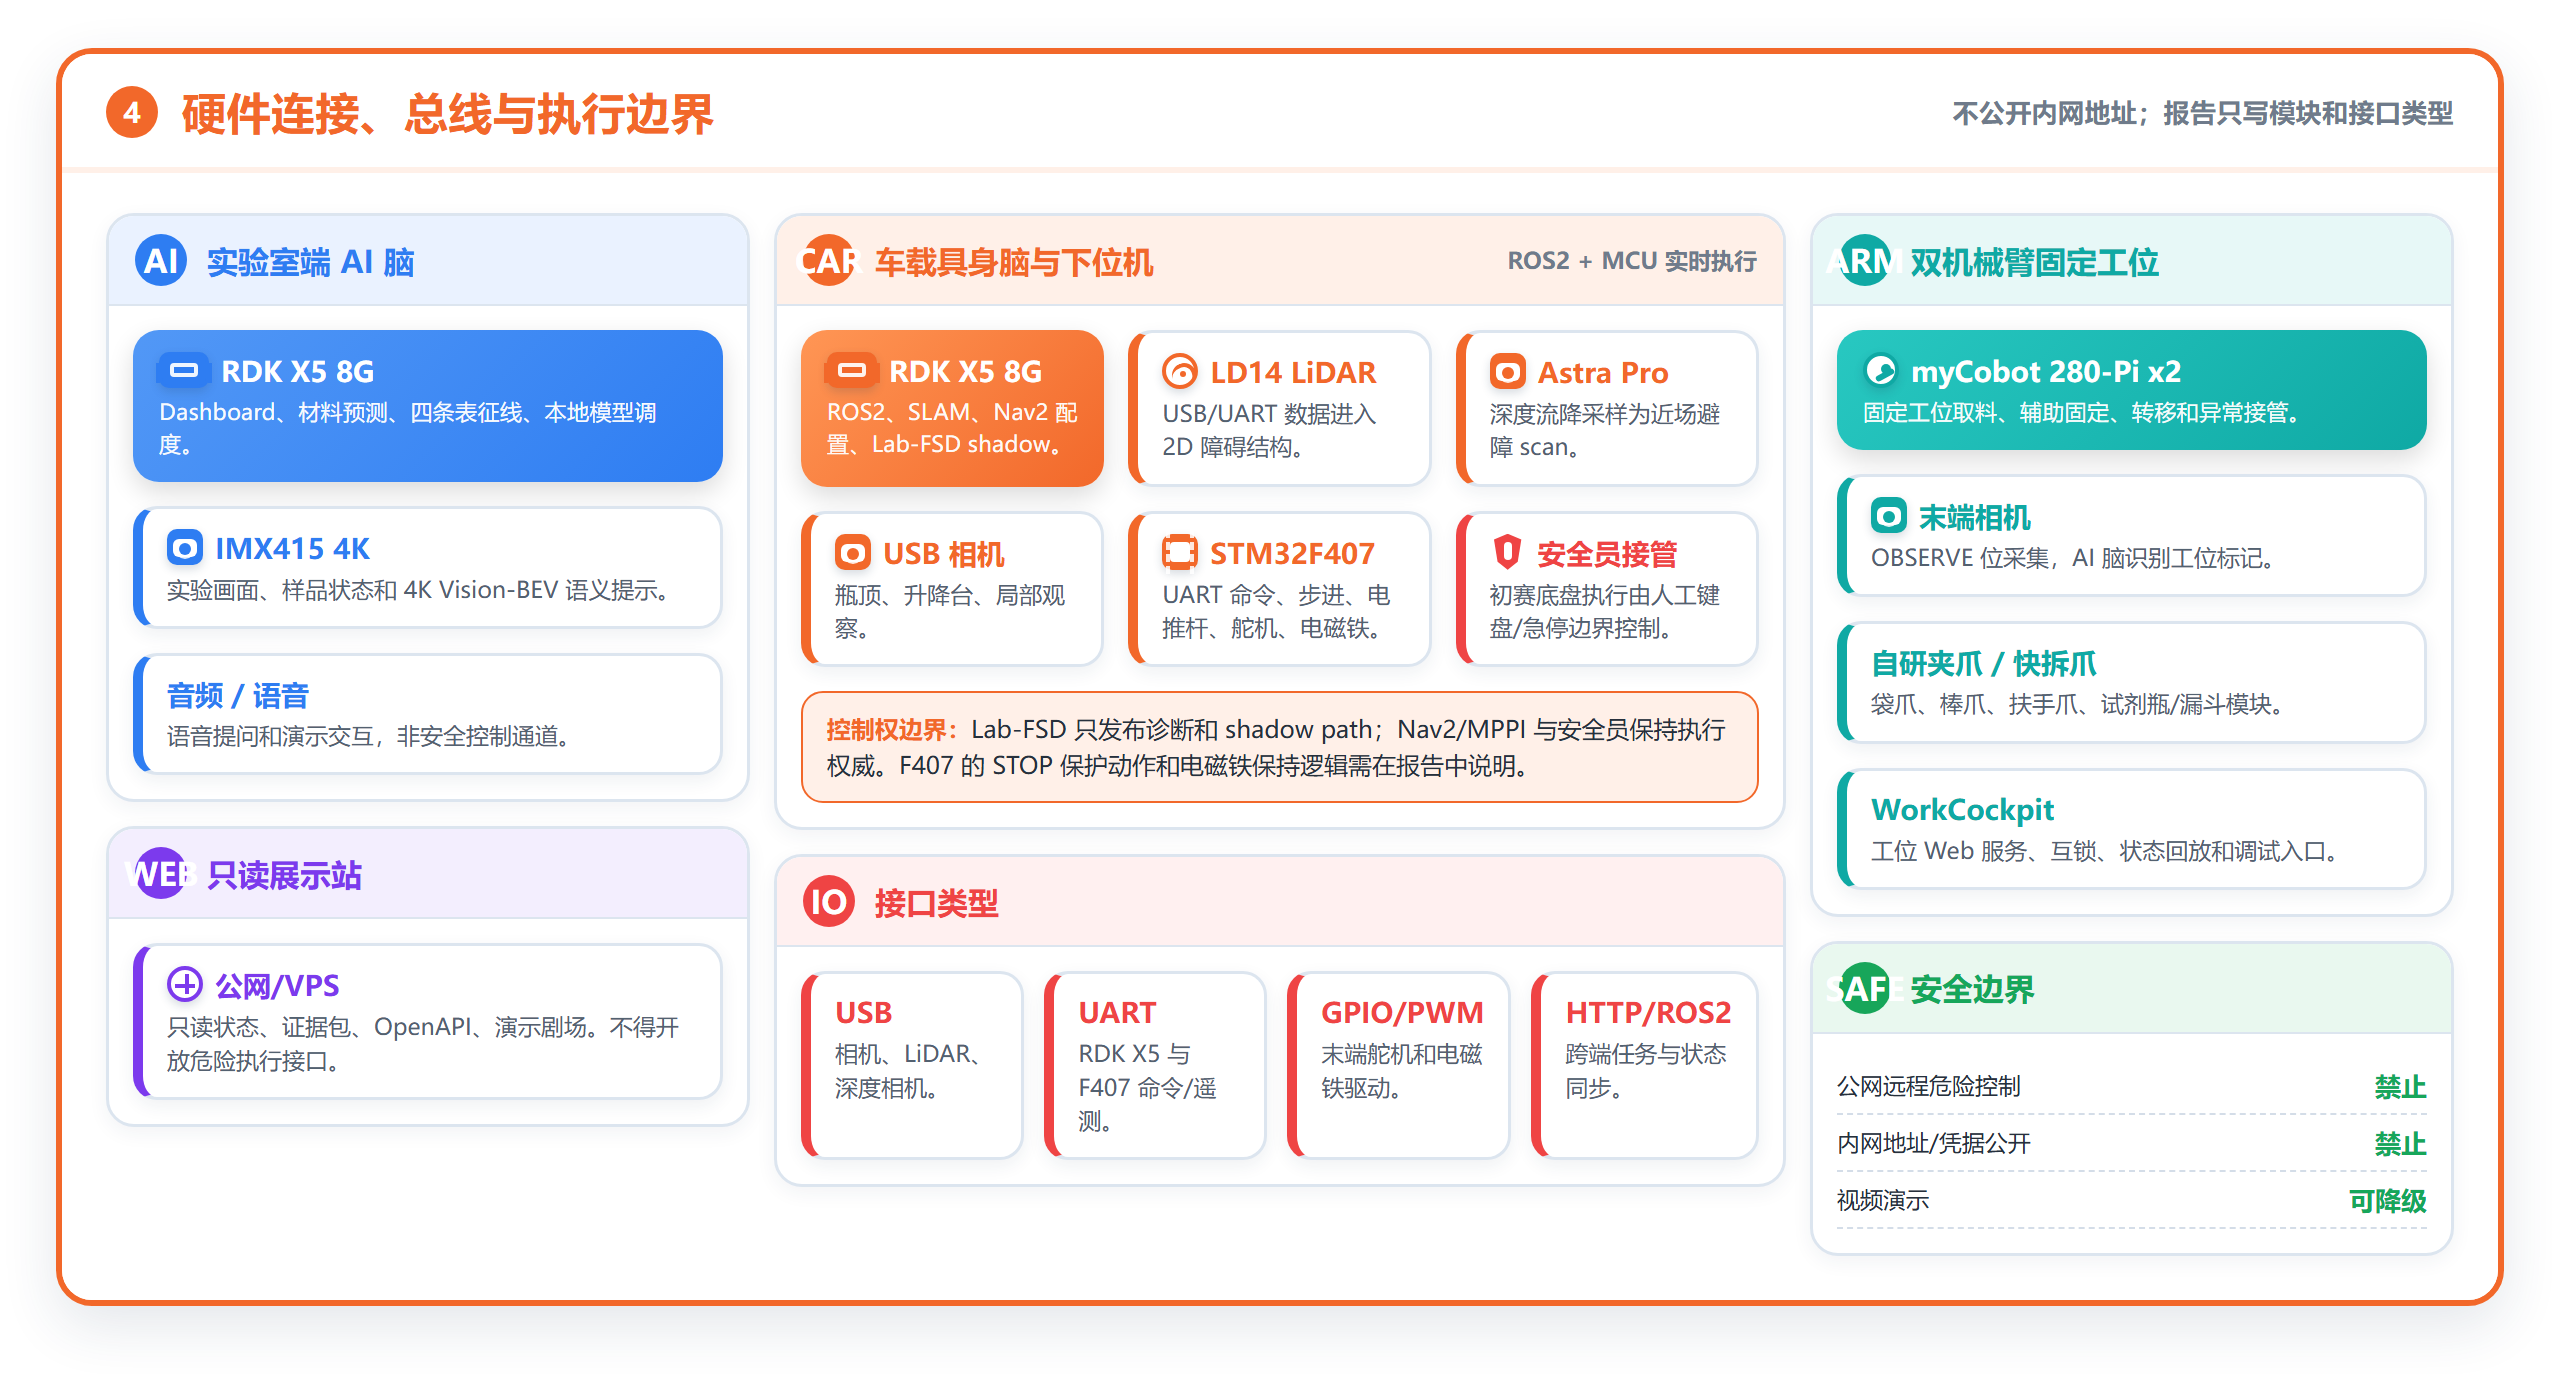
\includegraphics[width=\linewidth]{fig_xrd_hardware_html.png}
  \caption{硬件连接、总线与执行边界。}
  \label{fig:xrd_hardware}
\end{figure}

图~\ref{fig:xrd_hardware} 中不写具体内网地址、账号和凭据，只写模块和接口类型。这一处理同时满足竞赛匿名提交要求和项目保密要求。

\subsection{软件组成}
软件系统分为 AI 脑服务层、具身脑 ROS2 层、机械臂工位层、F407 固件层和公网证据层。AI 脑服务层负责材料预测、四条表征线和模型调度；具身脑 ROS2 层负责传感器驱动、SLAM、Lab-FSD 和诊断话题；机械臂工位层负责相机采集、示教位姿、PWM 夹爪和固定点动作；F407 固件层负责更接近实时的电机和电磁铁控制；公网证据层负责只读展示。

\begin{keybox}
系统的关键工程取舍是“高层智能与执行安全分离”。AI 脑可以给出材料建议和工位门控，具身脑可以给出风险和候选轨迹，但危险执行动作必须落到受控的本地节点、人工接管和硬件保护边界中。
\end{keybox}

\section{第二部分 系统组成及功能说明（三）：AI 脑与材料预测系统}

\subsection{五服务线架构}
AI 脑是实验室端嵌入式材料决策节点，不是网页平台。网页只是操作入口，核心能力在本地 X5 上：配方解析、材料预测、四条表征线接入、BPU/CPU 模型调度、失败规则过滤、实验记录追踪和 evidence package 输出。

\begin{figure}[H]
  \centering
  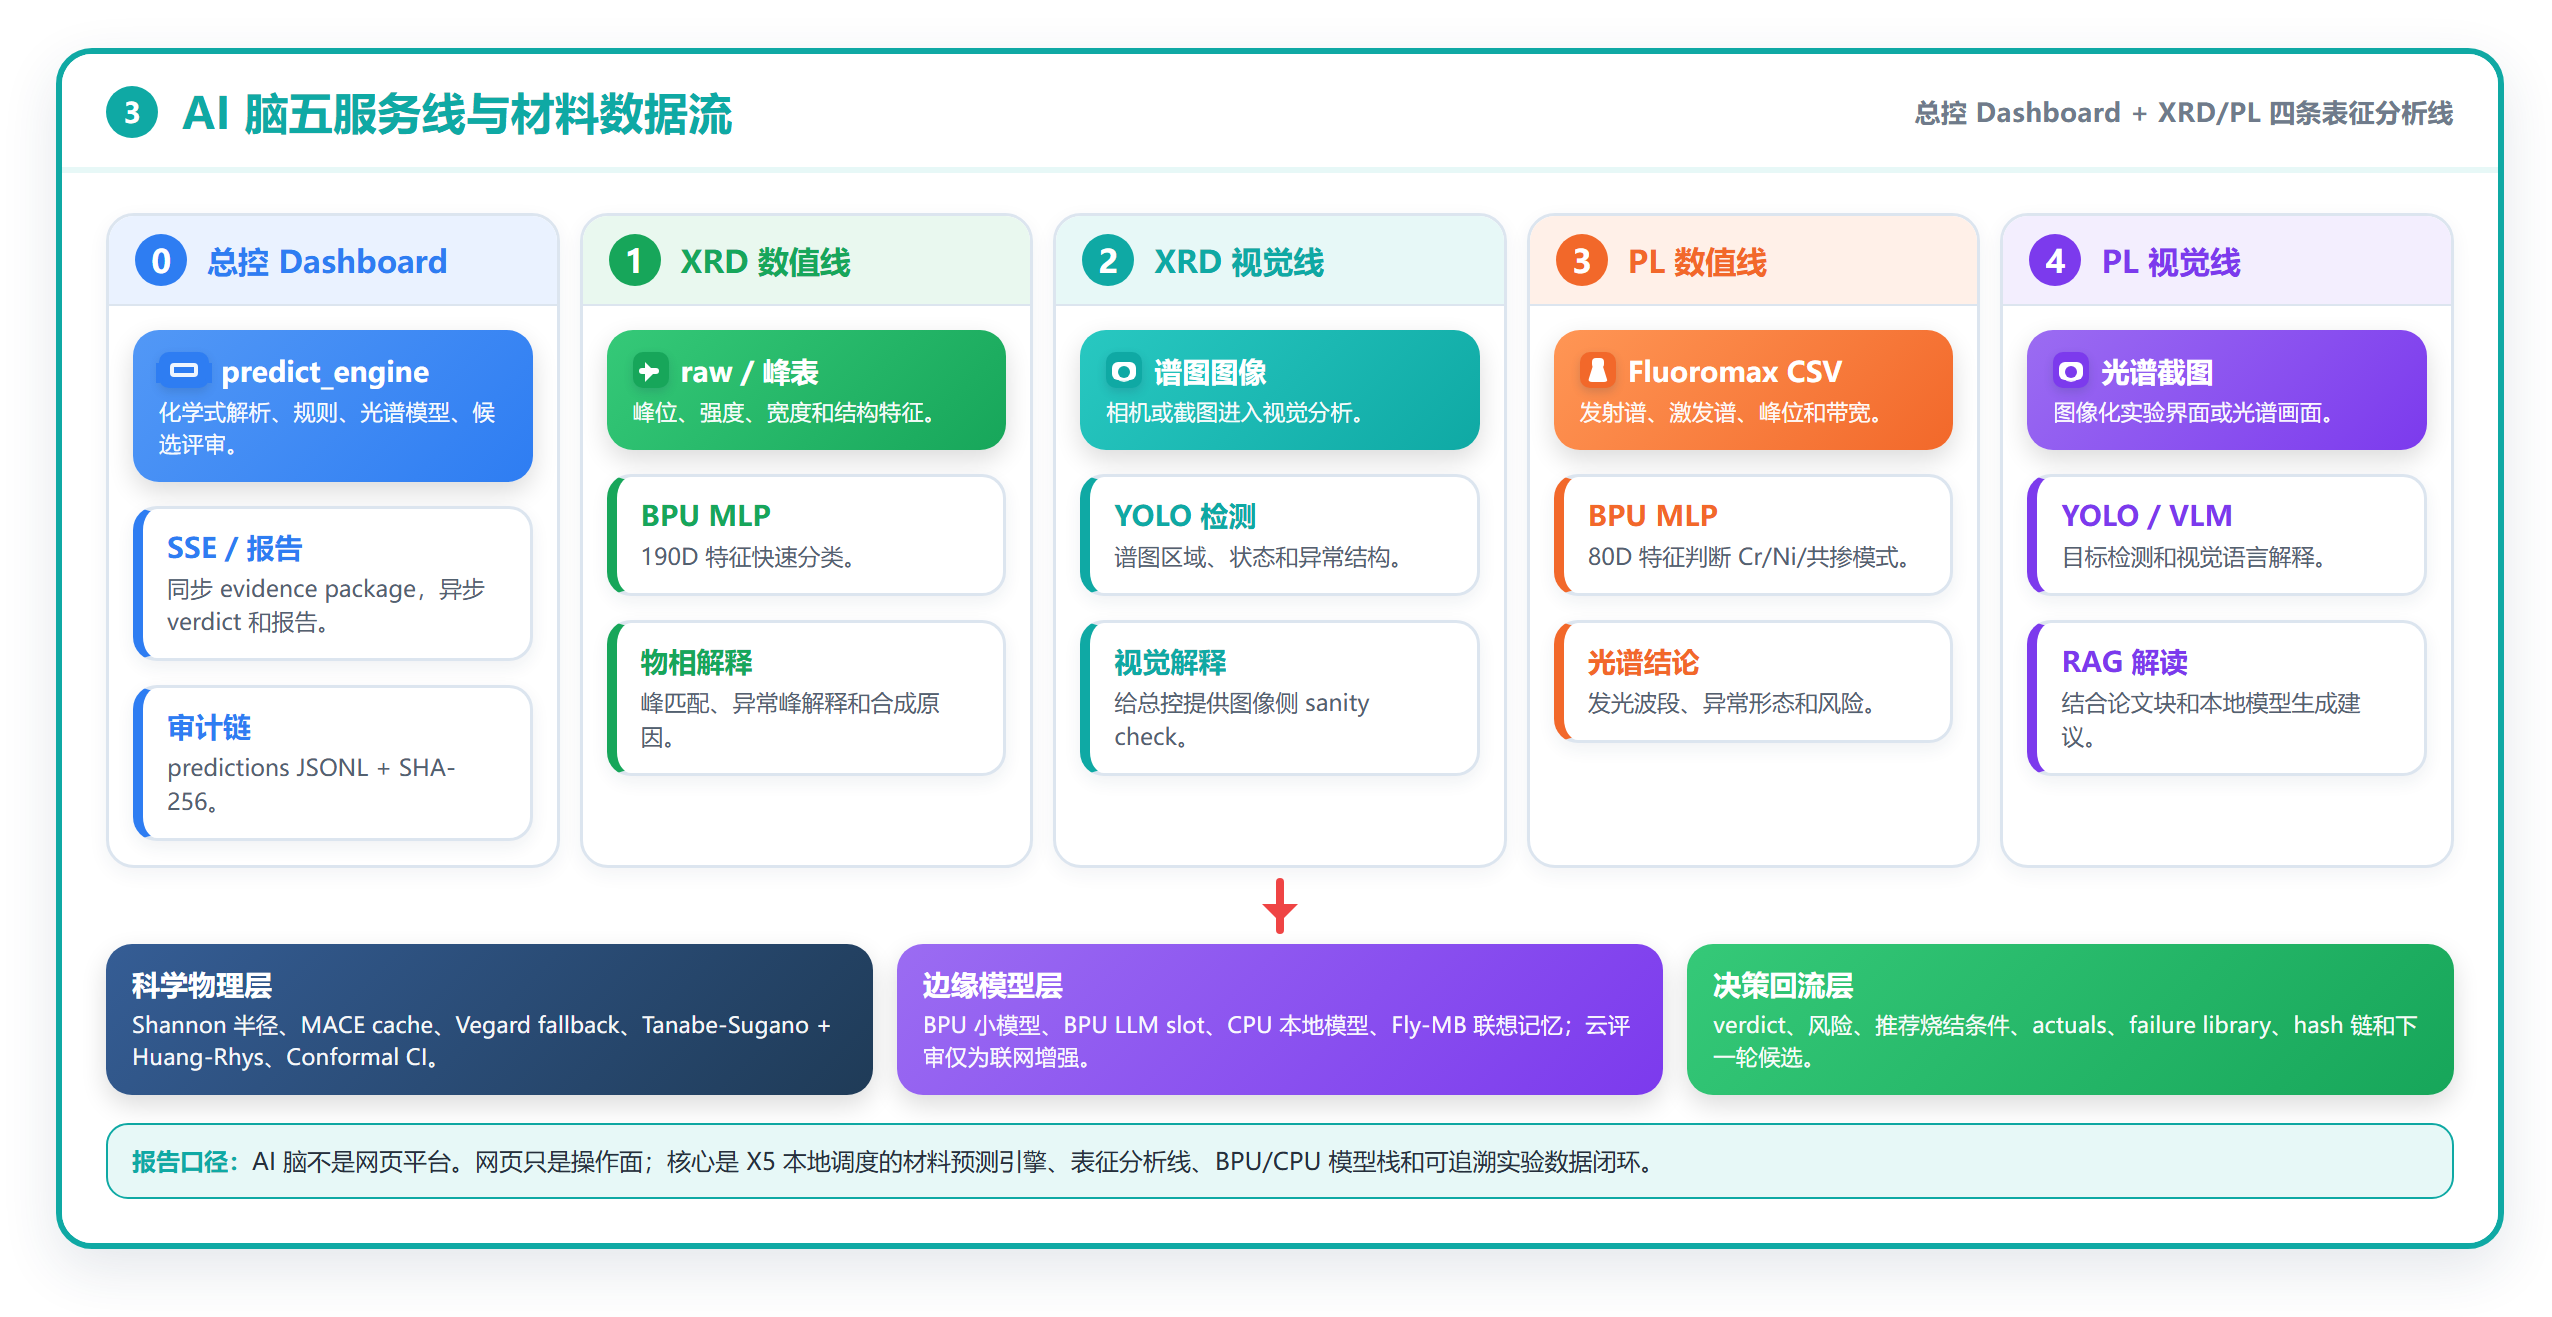
\includegraphics[width=\linewidth]{fig_xrd_dataflow_html.png}
  \caption{AI 脑五服务线与材料数据流。}
  \label{fig:xrd_dataflow}
\end{figure}

如图~\ref{fig:xrd_dataflow} 所示，五服务线包括总控 Dashboard、XRD 数值线、XRD 视觉线、PL 数值线和 PL 视觉线。数值线负责处理峰位、强度、带宽和结构特征；视觉线负责识别图像化谱图区域和实验状态；总控层把四条线的证据汇总到材料预测引擎。

\subsection{模型栈与决策层}
AI 脑模型栈分为三层：
\begin{itemize}
  \item \kw{科学物理层：} Shannon 半径、MACE 预计算缓存、Vegard fallback、Tanabe-Sugano + Huang-Rhys 光谱模型、Conformal CI 和实测类比库。
  \item \kw{边缘模型层：} BPU 轻量分类/检测模型、BPU LLM slot、CPU 本地模型和 Fly-MB 稀疏联想判决脑。
  \item \kw{决策回流层：} 同步 evidence package、异步 verdict、actuals 回填、failure library、Fly-MB plasticity 和 SHA-256 hash 链。
\end{itemize}

\begin{figure}[H]
  \centering
  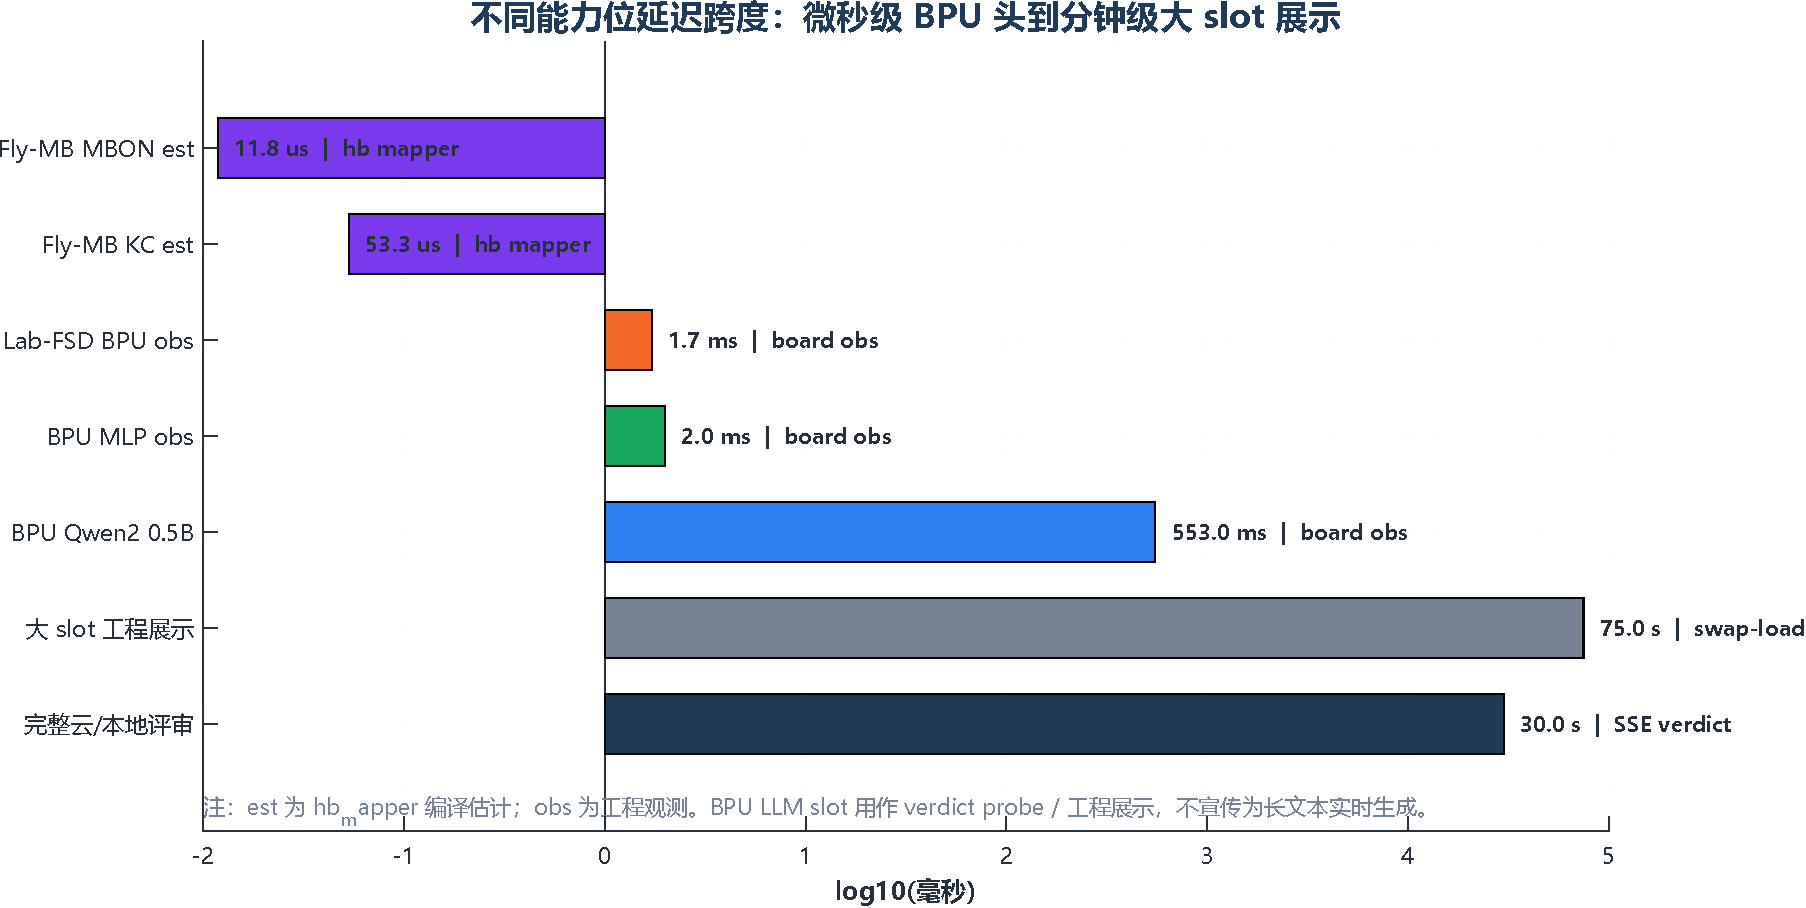
\includegraphics[width=0.96\linewidth]{fig_xrd_latency.pdf}
  \caption{不同模型能力位的延迟跨度与报告口径。}
  \label{fig:xrd_latency}
\end{figure}

图~\ref{fig:xrd_latency} 强调两个事实。第一，BPU 上的轻量头和小模型适合做毫秒级或更低延迟的结构化判断。第二，BPU LLM slot 适合作为 verdict probe 和工程展示，不应在报告中宣传为可实时长文本生成。完整材料解释由 CPU 本地模型、规则、知识库和可联网评审器共同完成。

\subsection{材料预测输出}
AI 脑对单个候选配方输出以下信息：
\begin{itemize}
  \item 候选 host、掺杂离子、位点、浓度和解析结果；
  \item 发光波段预测、可能峰位、置信区间和不确定性；
  \item GO / REVISE / DROP / UNKNOWN 等可行性判决；
  \item 风险来源，例如价态失配、半径失配、跨 host 外推或浓度淬灭；
  \item 推荐烧结温度、保温时间和后续实验建议；
  \item trace id、模型证据、规则证据和回填状态。
\end{itemize}

为了避免夸大，报告中将 MACE 写作“PC 端预计算的机器学习势能面结构弛豫缓存”，不写成 X5 端在线 DFT；将云模型写作联网增强评审器，不写成本地必需能力。

\section{第二部分 系统组成及功能说明（四）：具身脑、SLAM 与 Lab-FSD Shadow Planner}

\subsection{车载嵌入式执行子系统}
具身脑是车载嵌入式执行子系统。RDK X5 在车载侧运行 ROS2、传感器驱动、SLAM、Nav2 配置、BPU 感知和跨端桥接；STM32F407 负责更接近实时的电机、升降台、推杆、舵机和电磁铁控制。它不是遥控车，重点是端侧感知、状态机、MCU 执行和安全边界。

车载传感器中，LD14 LiDAR 是 SLAM 主传感器，Astra 深度相机提供近场深度扫描，里程计提供运动上下文，AI 脑的 4K Vision-BEV 提供语义风险提示但不替代 LiDAR、深度和里程计。

\subsection{Lab-FSD v2}
Lab-FSD v2 是低速实验室机器人场景下的 BEV 世界模型、影子规划和安全解释层。它订阅雷达、深度 scan、里程计、目标点和可选视觉 BEV，发布 BEV、future BEV、shadow path、policy tokens、risk、safety gate 等诊断信息。该模块明确不发布 \texttt{cmd\_vel}，安全门也标注 \texttt{cmd\_vel\_authority=false}。

\begin{figure}[H]
  \centering
  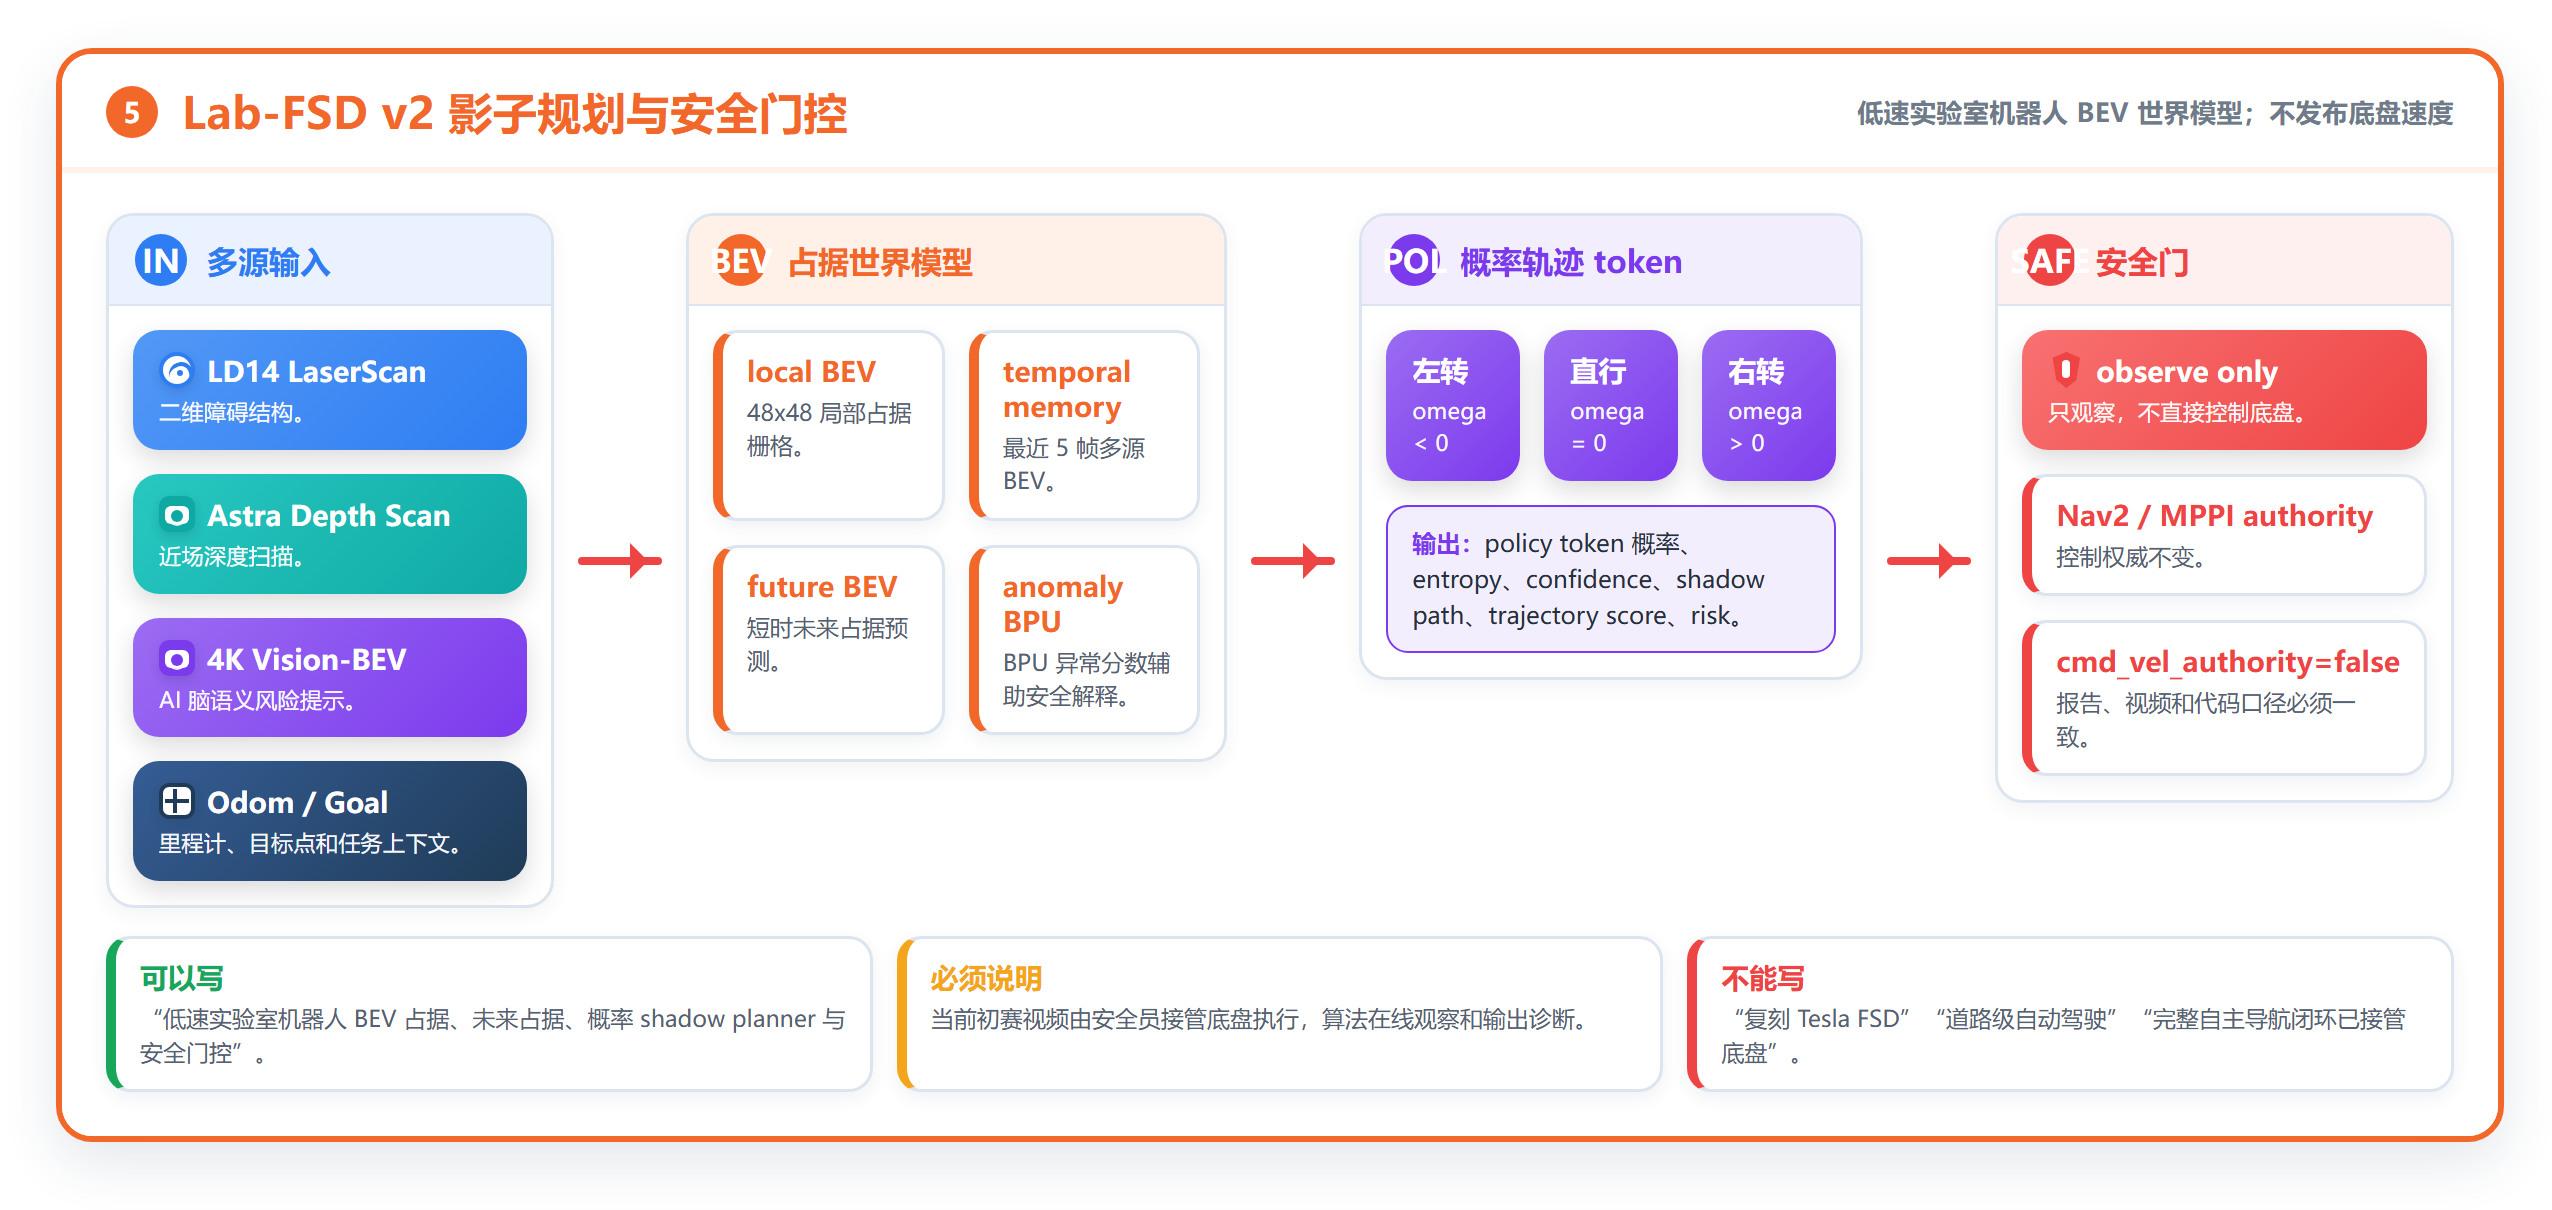
\includegraphics[width=\linewidth]{fig_xrd_labfsd_html.png}
  \caption{Lab-FSD v2 影子规划与安全门控。}
  \label{fig:xrd_labfsd}
\end{figure}

图~\ref{fig:xrd_labfsd} 是报告中的标准口径：可以说“低速实验室机器人 BEV 占据、未来占据、概率 shadow planner 与安全门控”，必须说明“当前初赛视频由安全员接管底盘执行，算法在线观察和输出诊断”，不能说“复刻自动驾驶”“道路级自动驾驶”或“完整自主导航已接管底盘”。

\subsection{SLAM 建图证据}
初赛现场已经跑通实验室 SLAM 占据栅格，后续将用于导航边界和安全门控初始化。

\begin{figure}[H]
  \centering
  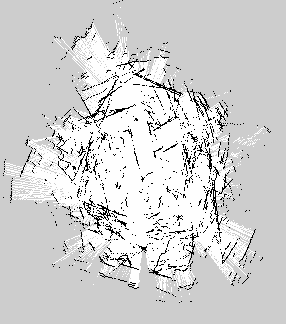
\includegraphics[width=0.72\linewidth]{fig_xrd_slam_map.png}
  \caption{实验室 SLAM 占据栅格建图结果。}
  \label{fig:xrd_slam}
\end{figure}

该图表明移动感知链路不是只停留在 PPT 或仿真层面，而是已经产生真实地图输出。由于初赛拍摄需要可控性，底盘执行仍由安全员接管，地图质量优化、Nav2 目标点和硬件安全保护作为后续闭环升级项。

\section{第二部分 系统组成及功能说明（五）：固定工位、机械臂与 F407 执行层}

\subsection{固定工位定位}
双 myCobot 固定工位是实验室执行单元，不是普通机械臂展示。它包含 Pi 侧机械臂控制、USB 末端相机、AprilTag/视觉门控、自研夹爪、WorkCockpit、示教位姿和回放证据。完整方案中，两台机械臂分别承担取料、辅助固定、转移和异常接管任务；初赛阶段重点展示 arm01 的视觉门控固定点取袋闭环和单臂冗余接管能力。

\begin{figure}[H]
  \centering
  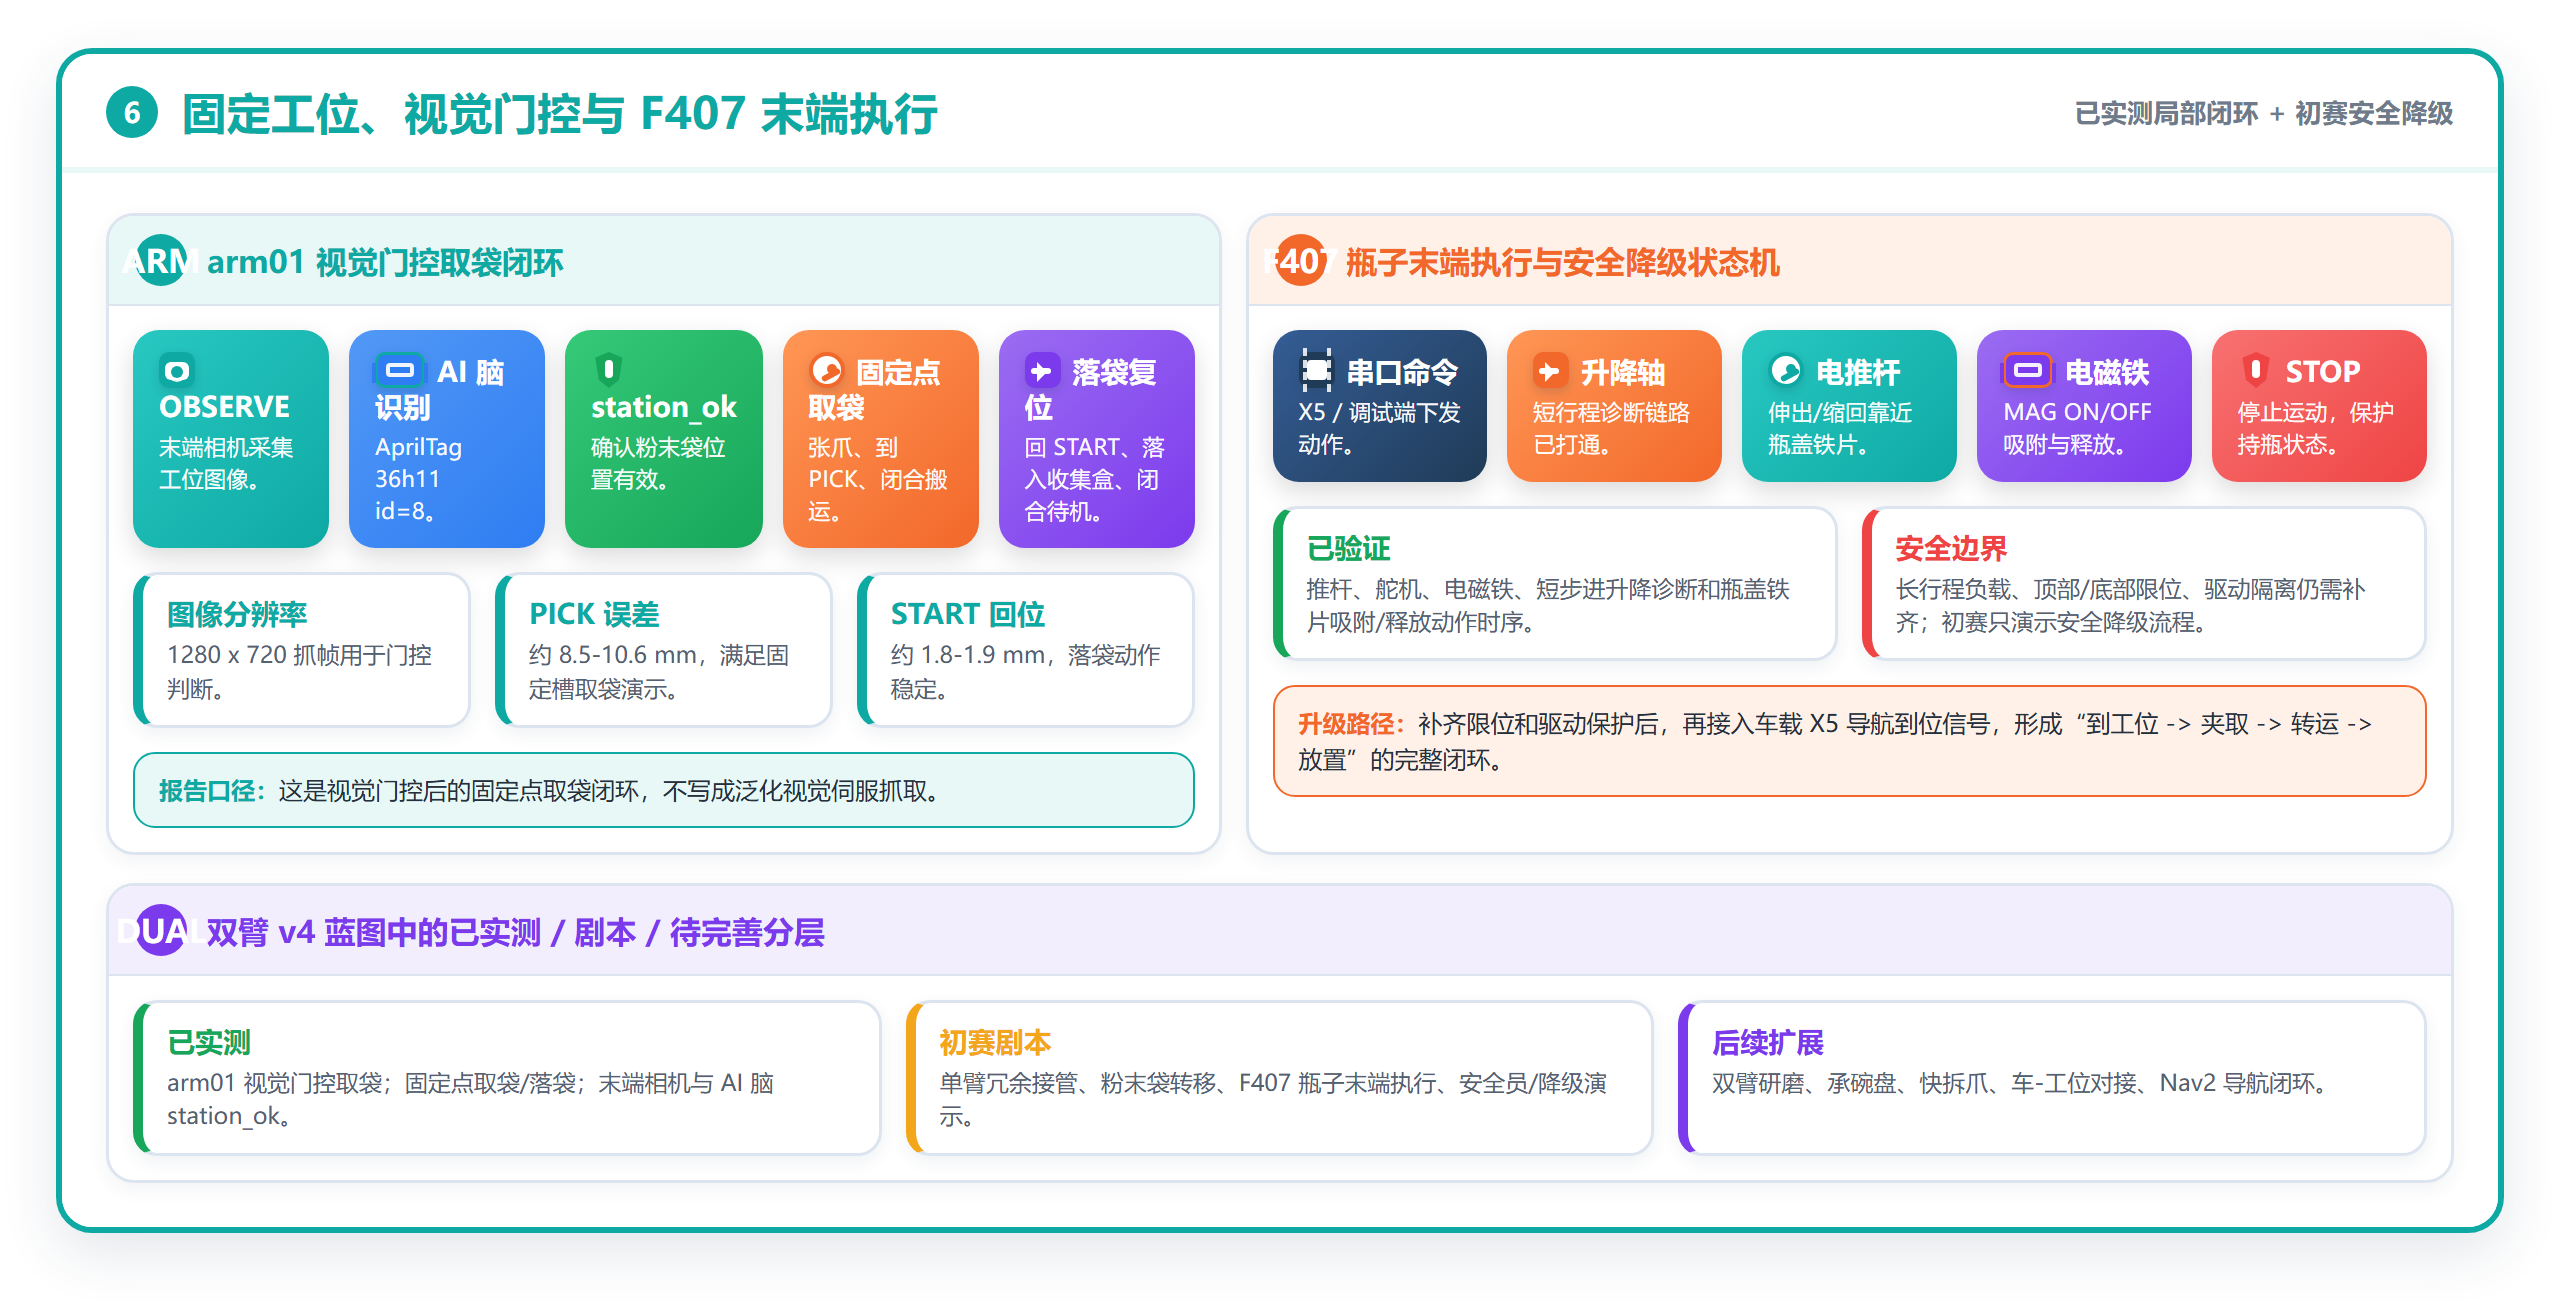
\includegraphics[width=\linewidth]{fig_xrd_workstation_html.png}
  \caption{固定工位、视觉门控与 F407 末端执行。}
  \label{fig:xrd_workstation}
\end{figure}

\subsection{arm01 视觉门控取袋}
arm01 已完成“OBSERVE 位拍照 -> AI 脑识别 AprilTag -> \texttt{station\_ok=true} -> 回 START -> 固定点取袋/落袋”的闭环。该结果可以写作视觉门控固定点取袋闭环，不能写作泛化视觉伺服抓取。实测记录包括 1280x720 抓帧、AprilTag 36h11 id=8、PICK 误差约 8.5-10.6 mm、START 回位约 1.8-1.9 mm，以及末端 G23 舵机开、闭、搬运保持值。

\subsection{STM32F407 末端执行}
F407 末端执行层已打通串口命令、推杆、舵机、电磁铁、短步进升降诊断和瓶盖铁片吸附/释放动作时序。视频中展示的是安全降级流程：先验证瓶子抓取、保持、释放和下位机动作时序，再在后续加入顶部/底部限位和电磁铁驱动隔离后接入车载 X5 导航到位信号。

\begin{warnbox}
F407 升降轴在负载长行程下仍需补齐限位、驱动保护和隔离设计。因此报告只写“末端执行链路与安全降级演示已跑通”，不写成无人值守完整取放闭环。
\end{warnbox}

\subsection{双臂 v4 蓝图}
v4 方案定义了从配方下发、车载取料、车-工位对接、双臂倒粉、研磨、故障冗余、灌装、送烧结、取烧结样到 XRD/PL 回填的十阶段剧本。报告中将其作为系统蓝图和后续扩展方向；初赛已实测的内容单独列出，避免把蓝图全部写成已完成真机闭环。

\section{第二部分 系统组成及功能说明（六）：公网展示站与证据链}

\subsection{平台定位}
公网展示站是只读证据门户，不是核心算法的替代品，也不是远程控制台。它把复杂系统中的状态、API、发布、演示剧场、全球对标、FSD 世界模型、机群和资产清单集中展示，使评审可以快速理解项目边界和工程证据。
站点包含总览、亮点、答辩防御、全球对标、FSD 世界模型、机群和资产等页面。总览页展示现场两块 RDK X5、主机械臂、初赛单臂冗余演示和闭环路径；亮点页展示 AI 脑、具身脑、导航、取料和实验数据回流；答辩防御页用于解释技术可信度和边界；全球对标页把项目与公开顶级平台按维度对照；FSD 世界模型页展示实验室执行过程的可观察、可回放、可审计状态。

\begin{figure}[H]
  \centering
  \begin{subfigure}[t]{0.32\linewidth}
    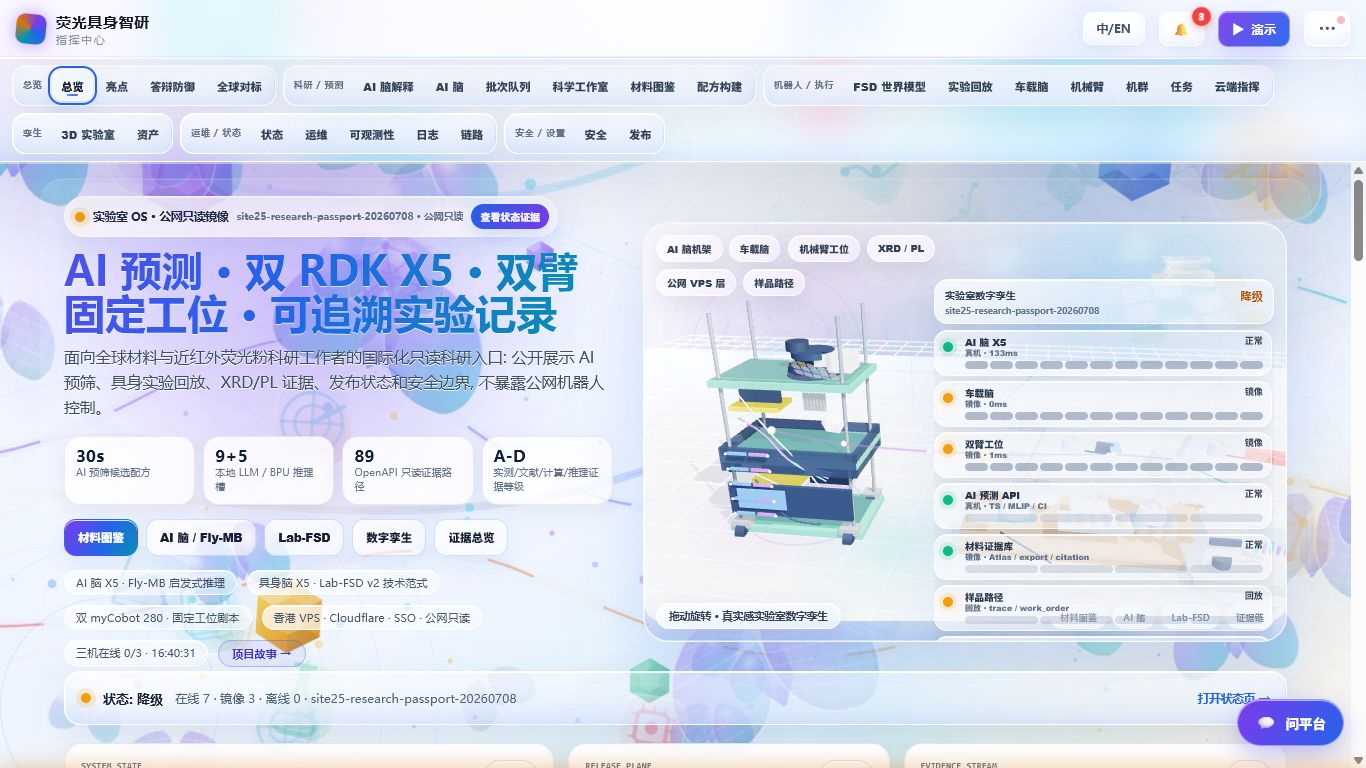
\includegraphics[width=\linewidth]{fig_xrd_site_home.png}
    \caption{总览与 OS 控制面}
  \end{subfigure}
  \hfill
  \begin{subfigure}[t]{0.32\linewidth}
    
\includegraphics[width=\linewidth]{fig_xrd_site_benchmark.png}
    \caption{全球对标}
  \end{subfigure}
  \hfill
  \begin{subfigure}[t]{0.32\linewidth}
    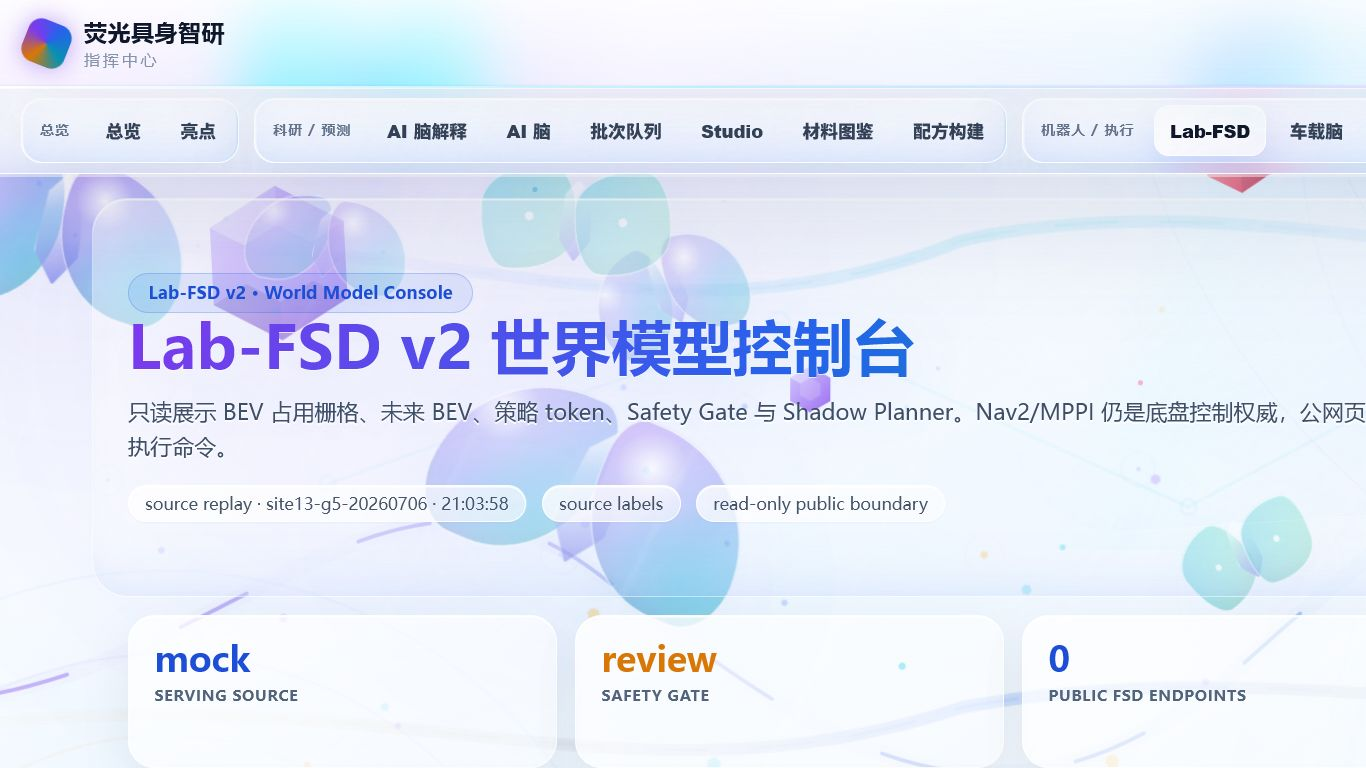
\includegraphics[width=\linewidth]{fig_xrd_site_fsd.png}
    \caption{FSD 世界模型}
  \end{subfigure}
  \caption{公网展示站真实页面截图。}
  \label{fig:xrd_site}
\end{figure}

\subsection{证据链组成}
证据链包括四类内容：
\begin{enumerate}
  \item \kw{算法证据：} 模型栈、BPU/CPU 能力位、预测 trace、evidence package 和报告页。
  \item \kw{执行证据：} SLAM 地图、Lab-FSD topic、arm01 取袋记录、F407 动作时序。
  \item \kw{工程证据：} OpenAPI paths、release、部署状态、hardening checks 和只读边界。
  \item \kw{提交证据：} 视频脚本、报告、重要代码包、关键词和 GitHub 字段说明。
\end{enumerate}

\begin{keybox}
公网平台的安全原则是只读展示。报告和代码包中不得包含可直接控制底盘、机械臂、升降台、电磁铁或舵机的公网入口。
\end{keybox}

\section{第三部分 完成情况及性能参数}

本部分按照“最终实现成果以图文结合说明、实物照片为主”的要求组织。项目当前已形成由双 RDK X5、车载具身平台、双 myCobot 固定工位和 STM32F407 末端执行层组成的材料实验助理机器人样机。初赛阶段采用安全员接管底盘、规划与感知在线 shadow mode、末端执行分段验证的展示方式，重点证明系统工程链路已经跑通，而不是只给出软件页面或单一传感器演示。

\subsection*{3.1 整体介绍}
\phantomsection
\addcontentsline{toc}{subsection}{3.1 整体介绍}

图~\ref{fig:actual_system_global} 为当前系统的全局实物照片。左侧为车载具身脑平台，包含 RDK X5、LD14 激光雷达、Astra 深度相机、小米云台/USB 摄像头、升降与瓶子吸附执行机构、STM32F407 底层控制板、电源与电机驱动模块；右侧为固定实验工位，布置双 myCobot 280-Pi、末端摄像头、自研夹爪、粉末袋工位、转运盘和收集区域。系统整体按“AI 脑做材料预测与语义理解、具身脑做移动感知与规划、工位机械臂做取放执行、F407 做底层闭环动作”的异构协同方式工作。

\begin{figure}[H]
  \centering
  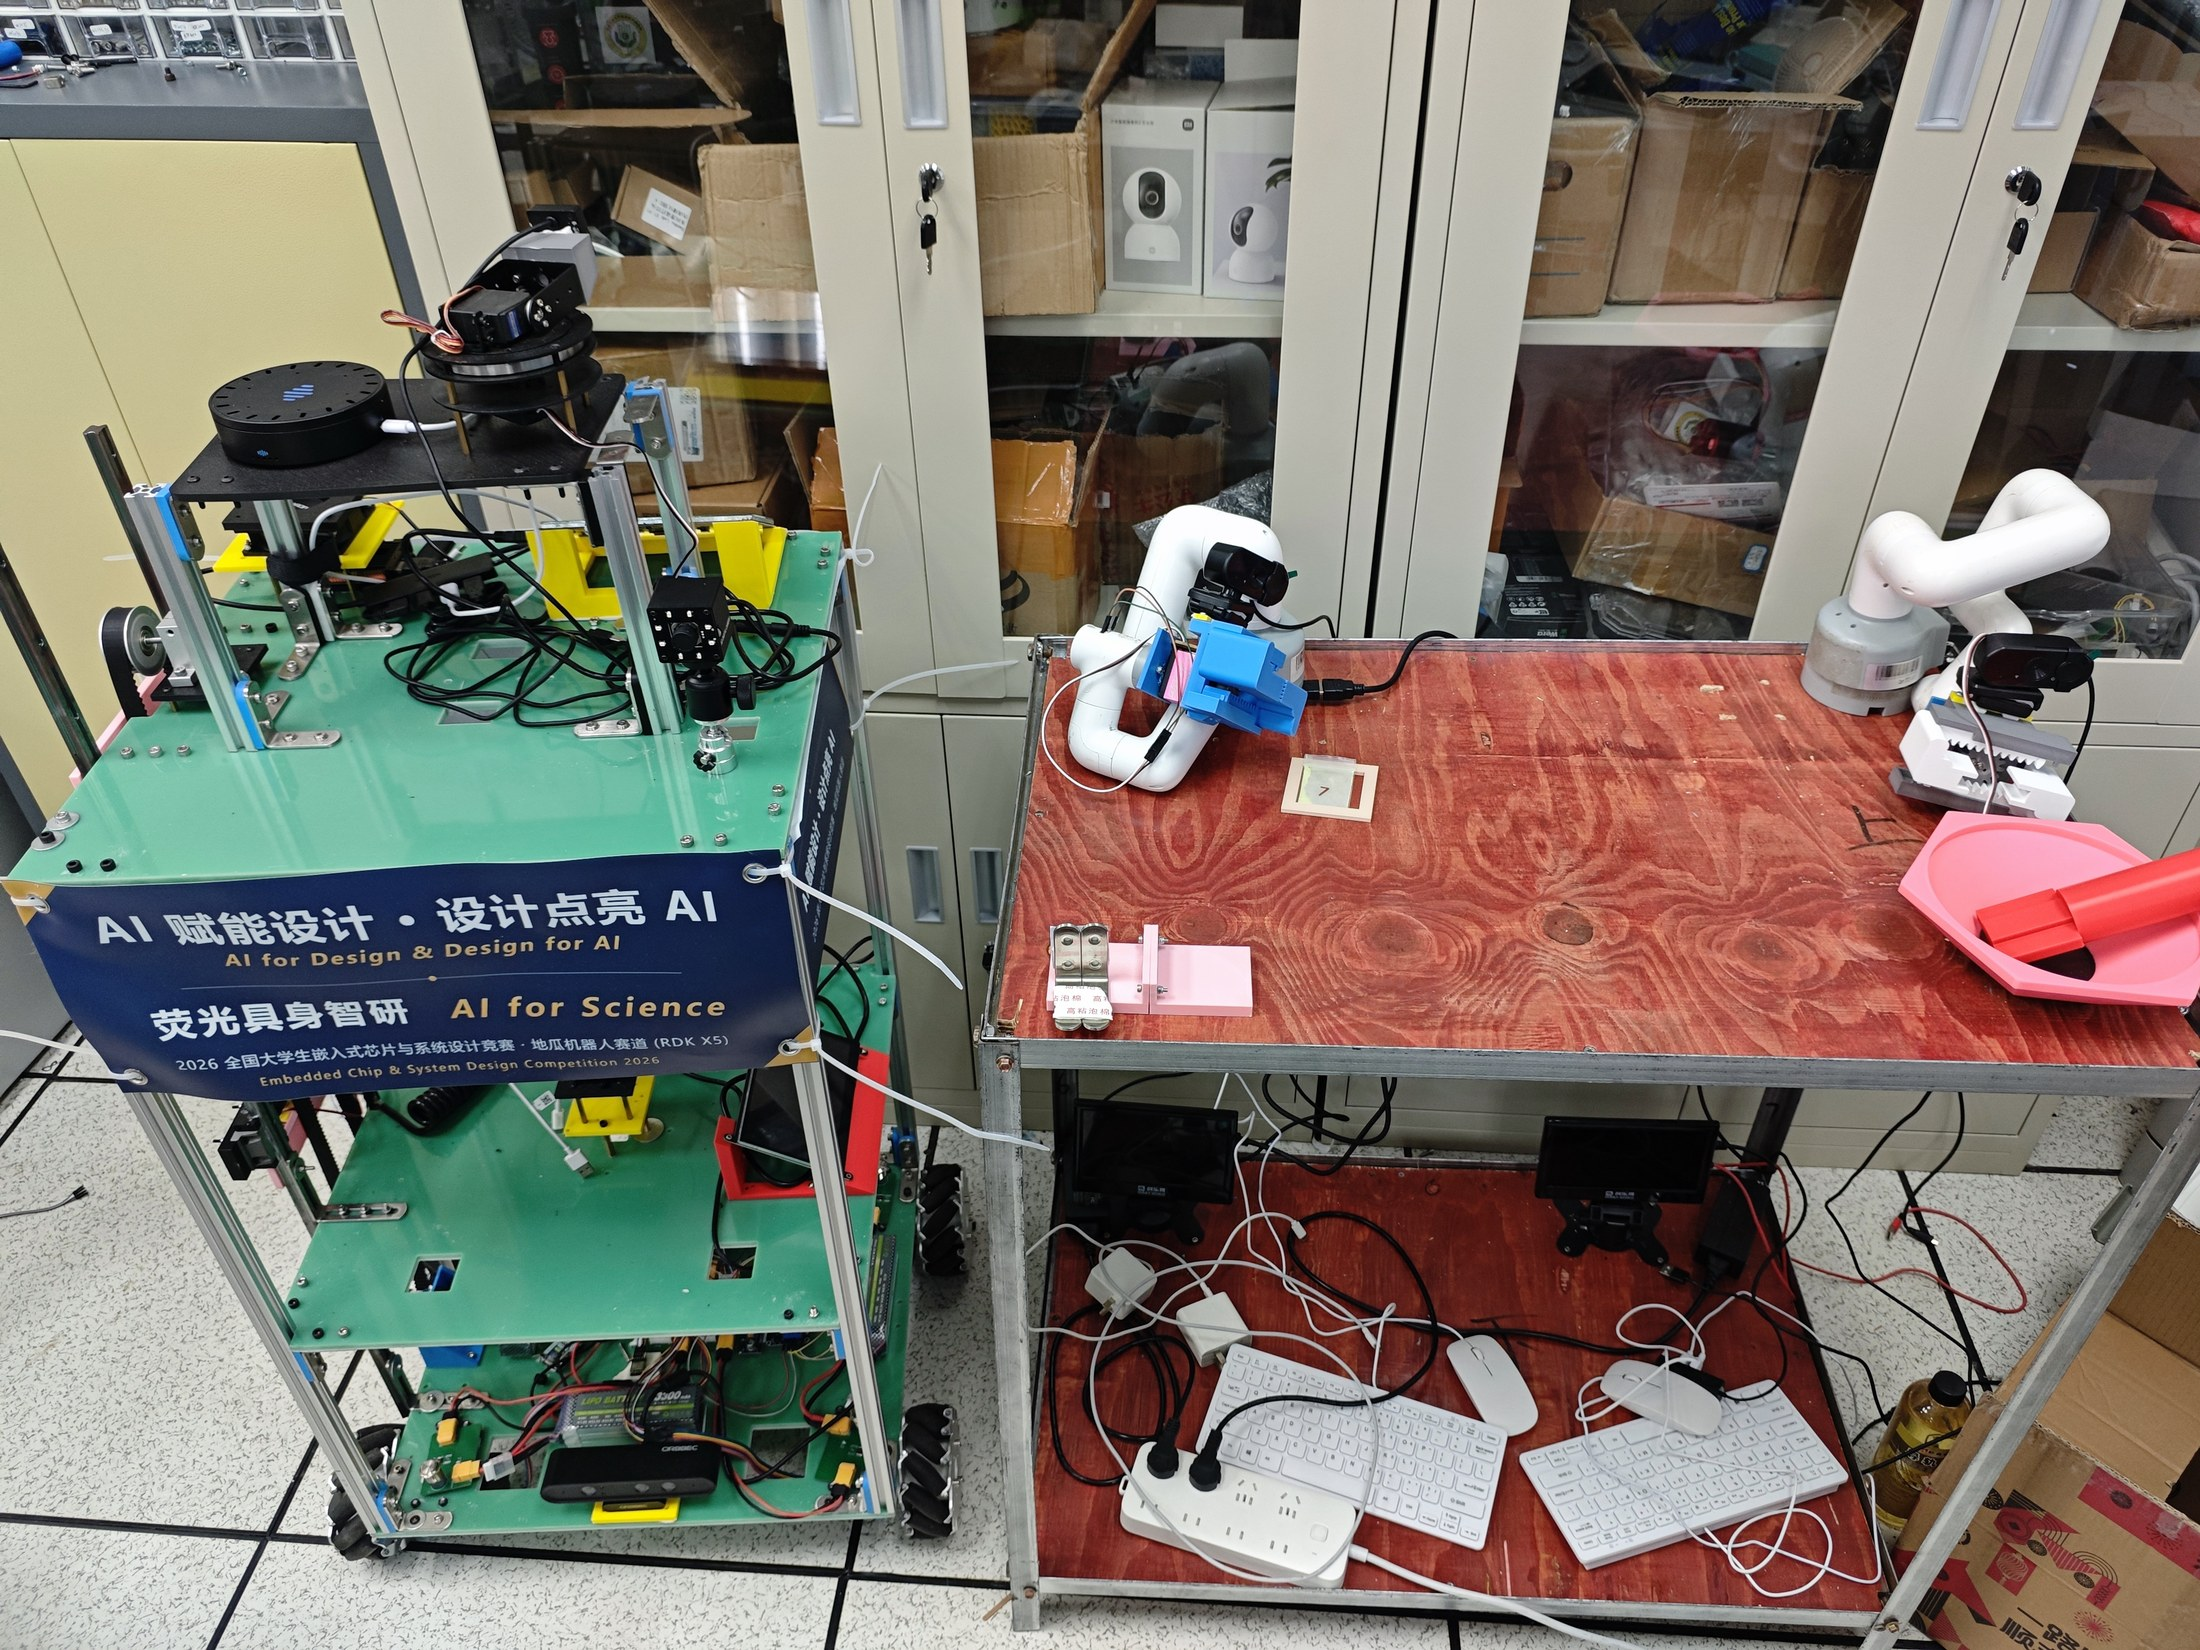
\includegraphics[width=0.98\linewidth]{fig_actual_system_global.jpg}
  \caption{系统实物全局照片：左侧为车载具身脑平台，右侧为双机械臂固定实验工位。}
  \label{fig:actual_system_global}
\end{figure}

\subsection*{3.2 工程成果}
\phantomsection
\addcontentsline{toc}{subsection}{3.2 工程成果}

\subsubsection*{3.2.1 机械成果}
\phantomsection
\addcontentsline{toc}{subsubsection}{3.2.1 机械成果}

机械部分已经完成车载平台、升降台、瓶子吸附机构、双臂固定工位和两类实验材料末端执行器的实物搭建。车载平台采用多层板式结构承载传感器、算力板、电源与执行机构；固定工位采用桌面式双臂布局，一侧机械臂可在另一侧异常或暂不可用时执行单臂冗余接管。末端夹爪面向薄片状粉末袋设计，瓶子执行端则采用“瓶盖铁片 + 电磁铁吸附 + 电推杆伸缩”的安全降级验证流程。

\begin{figure}[H]
  \centering
  \begin{subfigure}{0.42\linewidth}
    \centering
    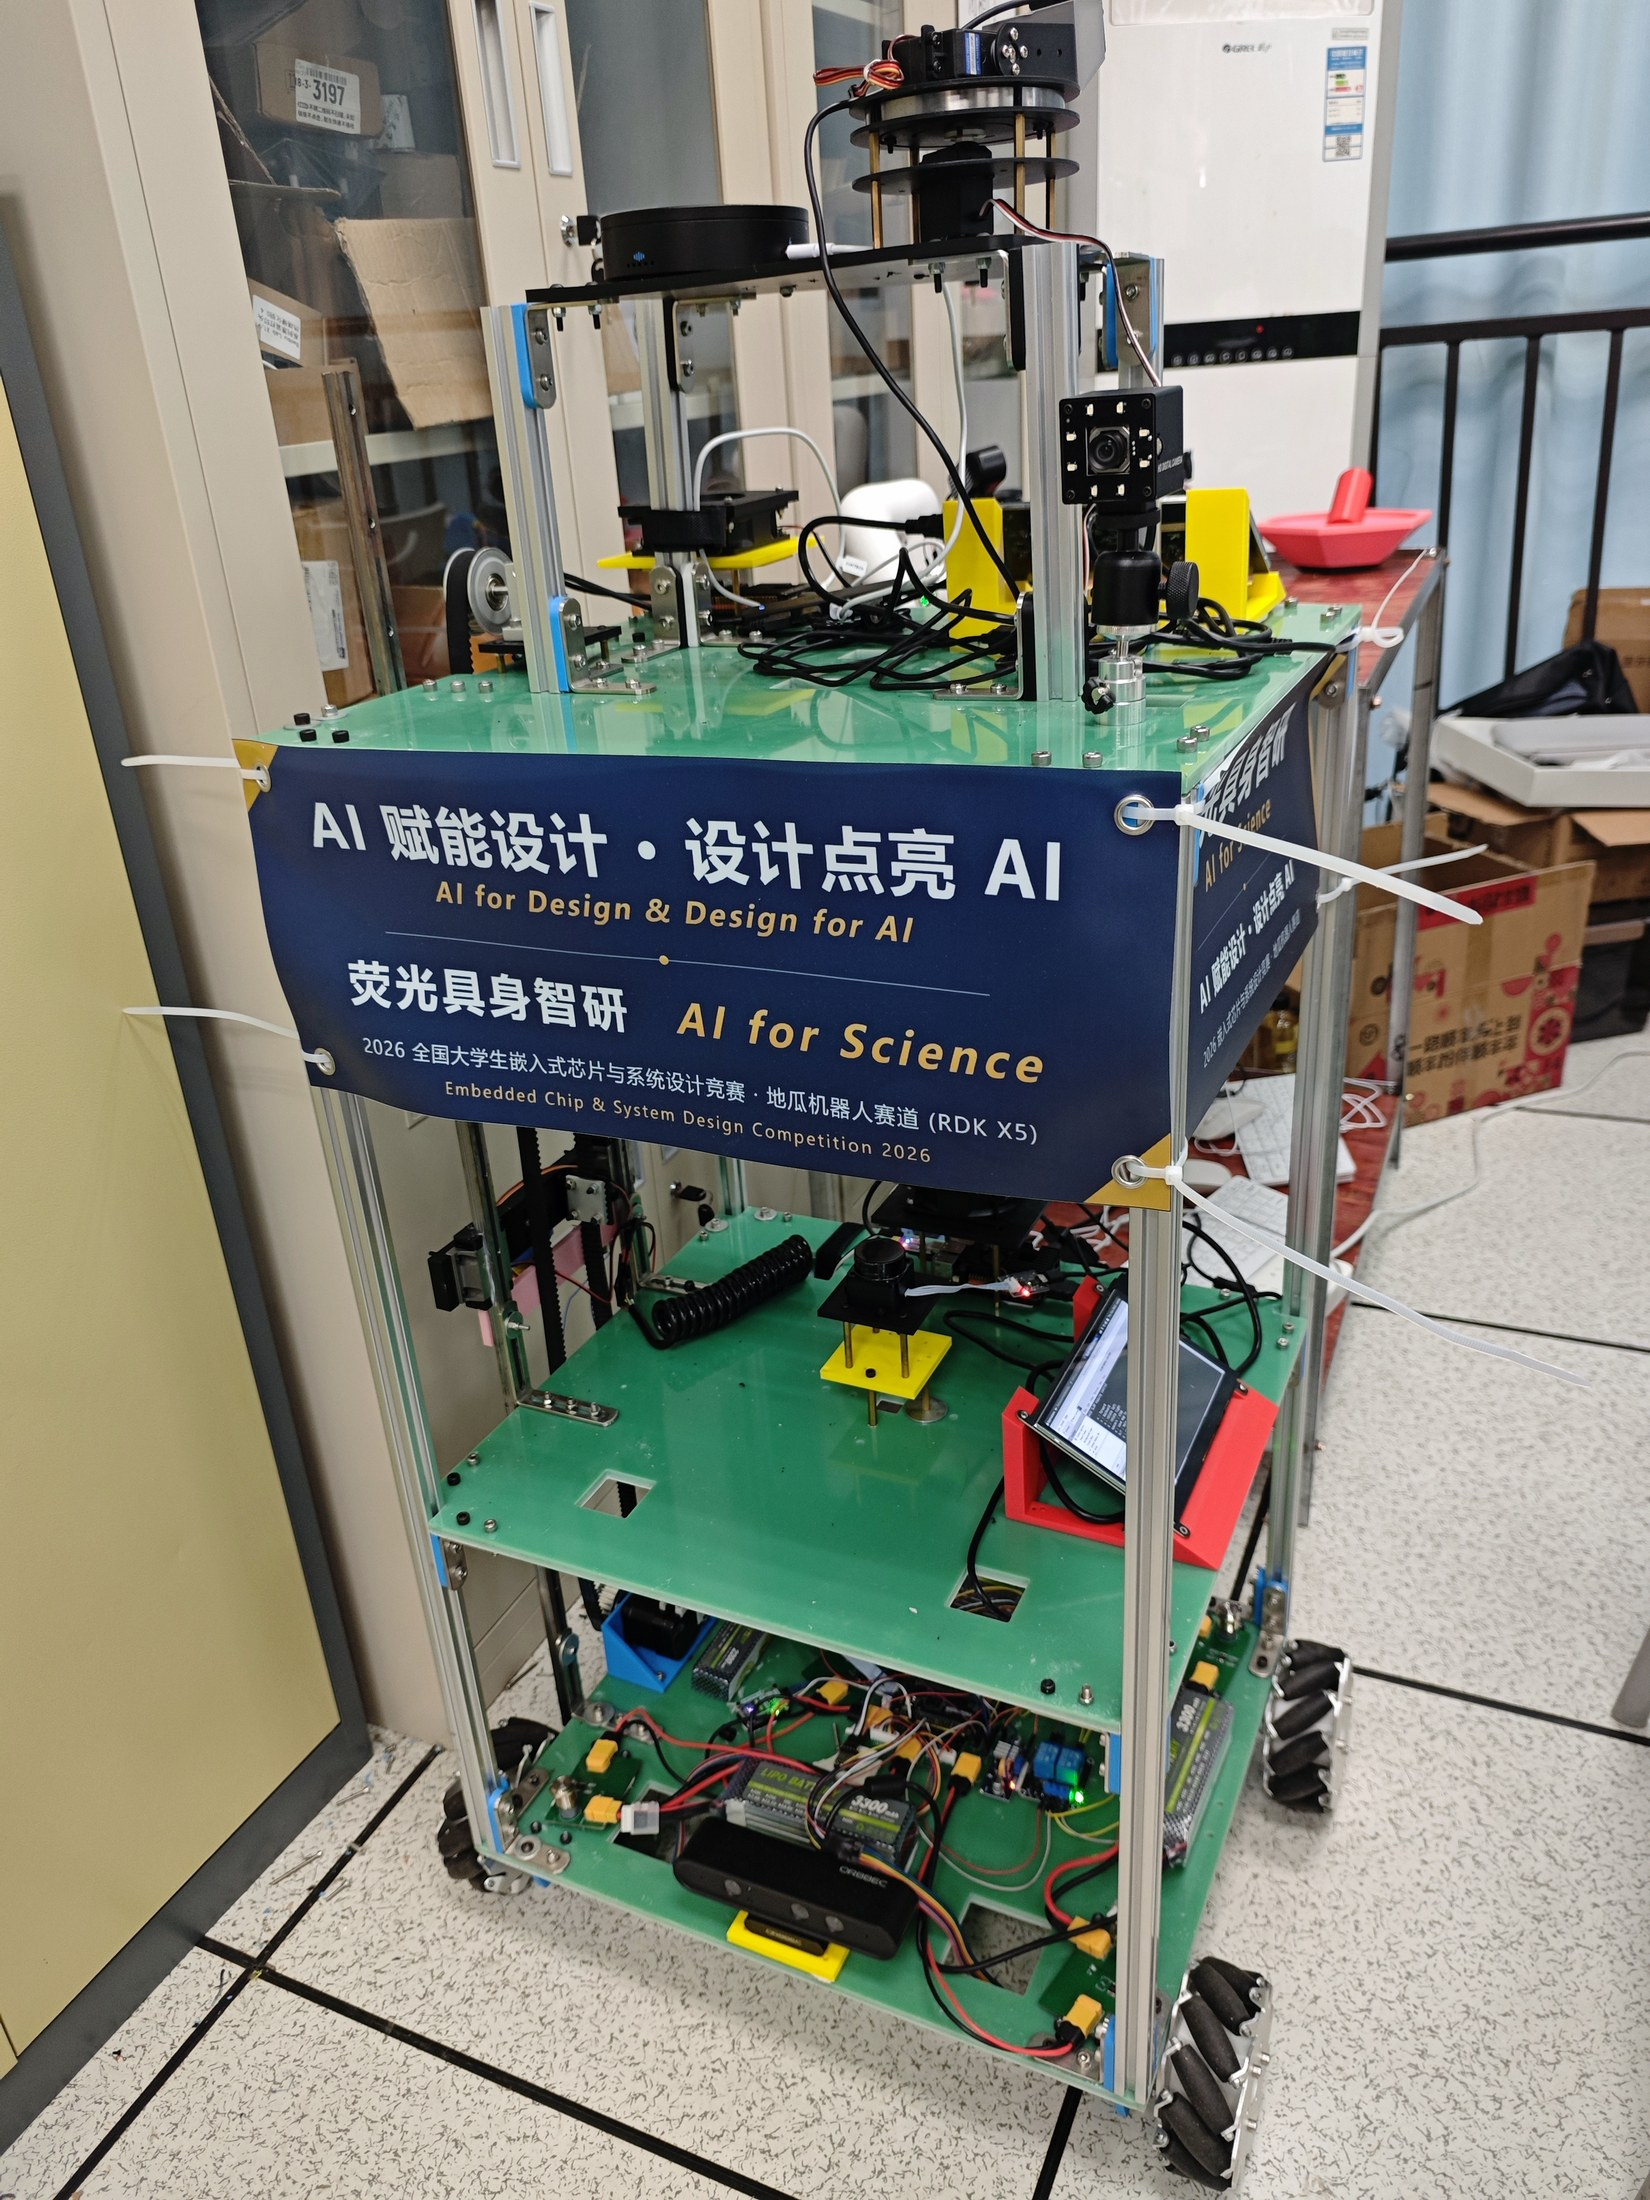
\includegraphics[width=\linewidth]{fig_actual_mech_car.jpg}
    \caption{车载平台、升降机构、传感器和执行机构。}
  \end{subfigure}
  \hfill
  \begin{subfigure}{0.54\linewidth}
    \centering
    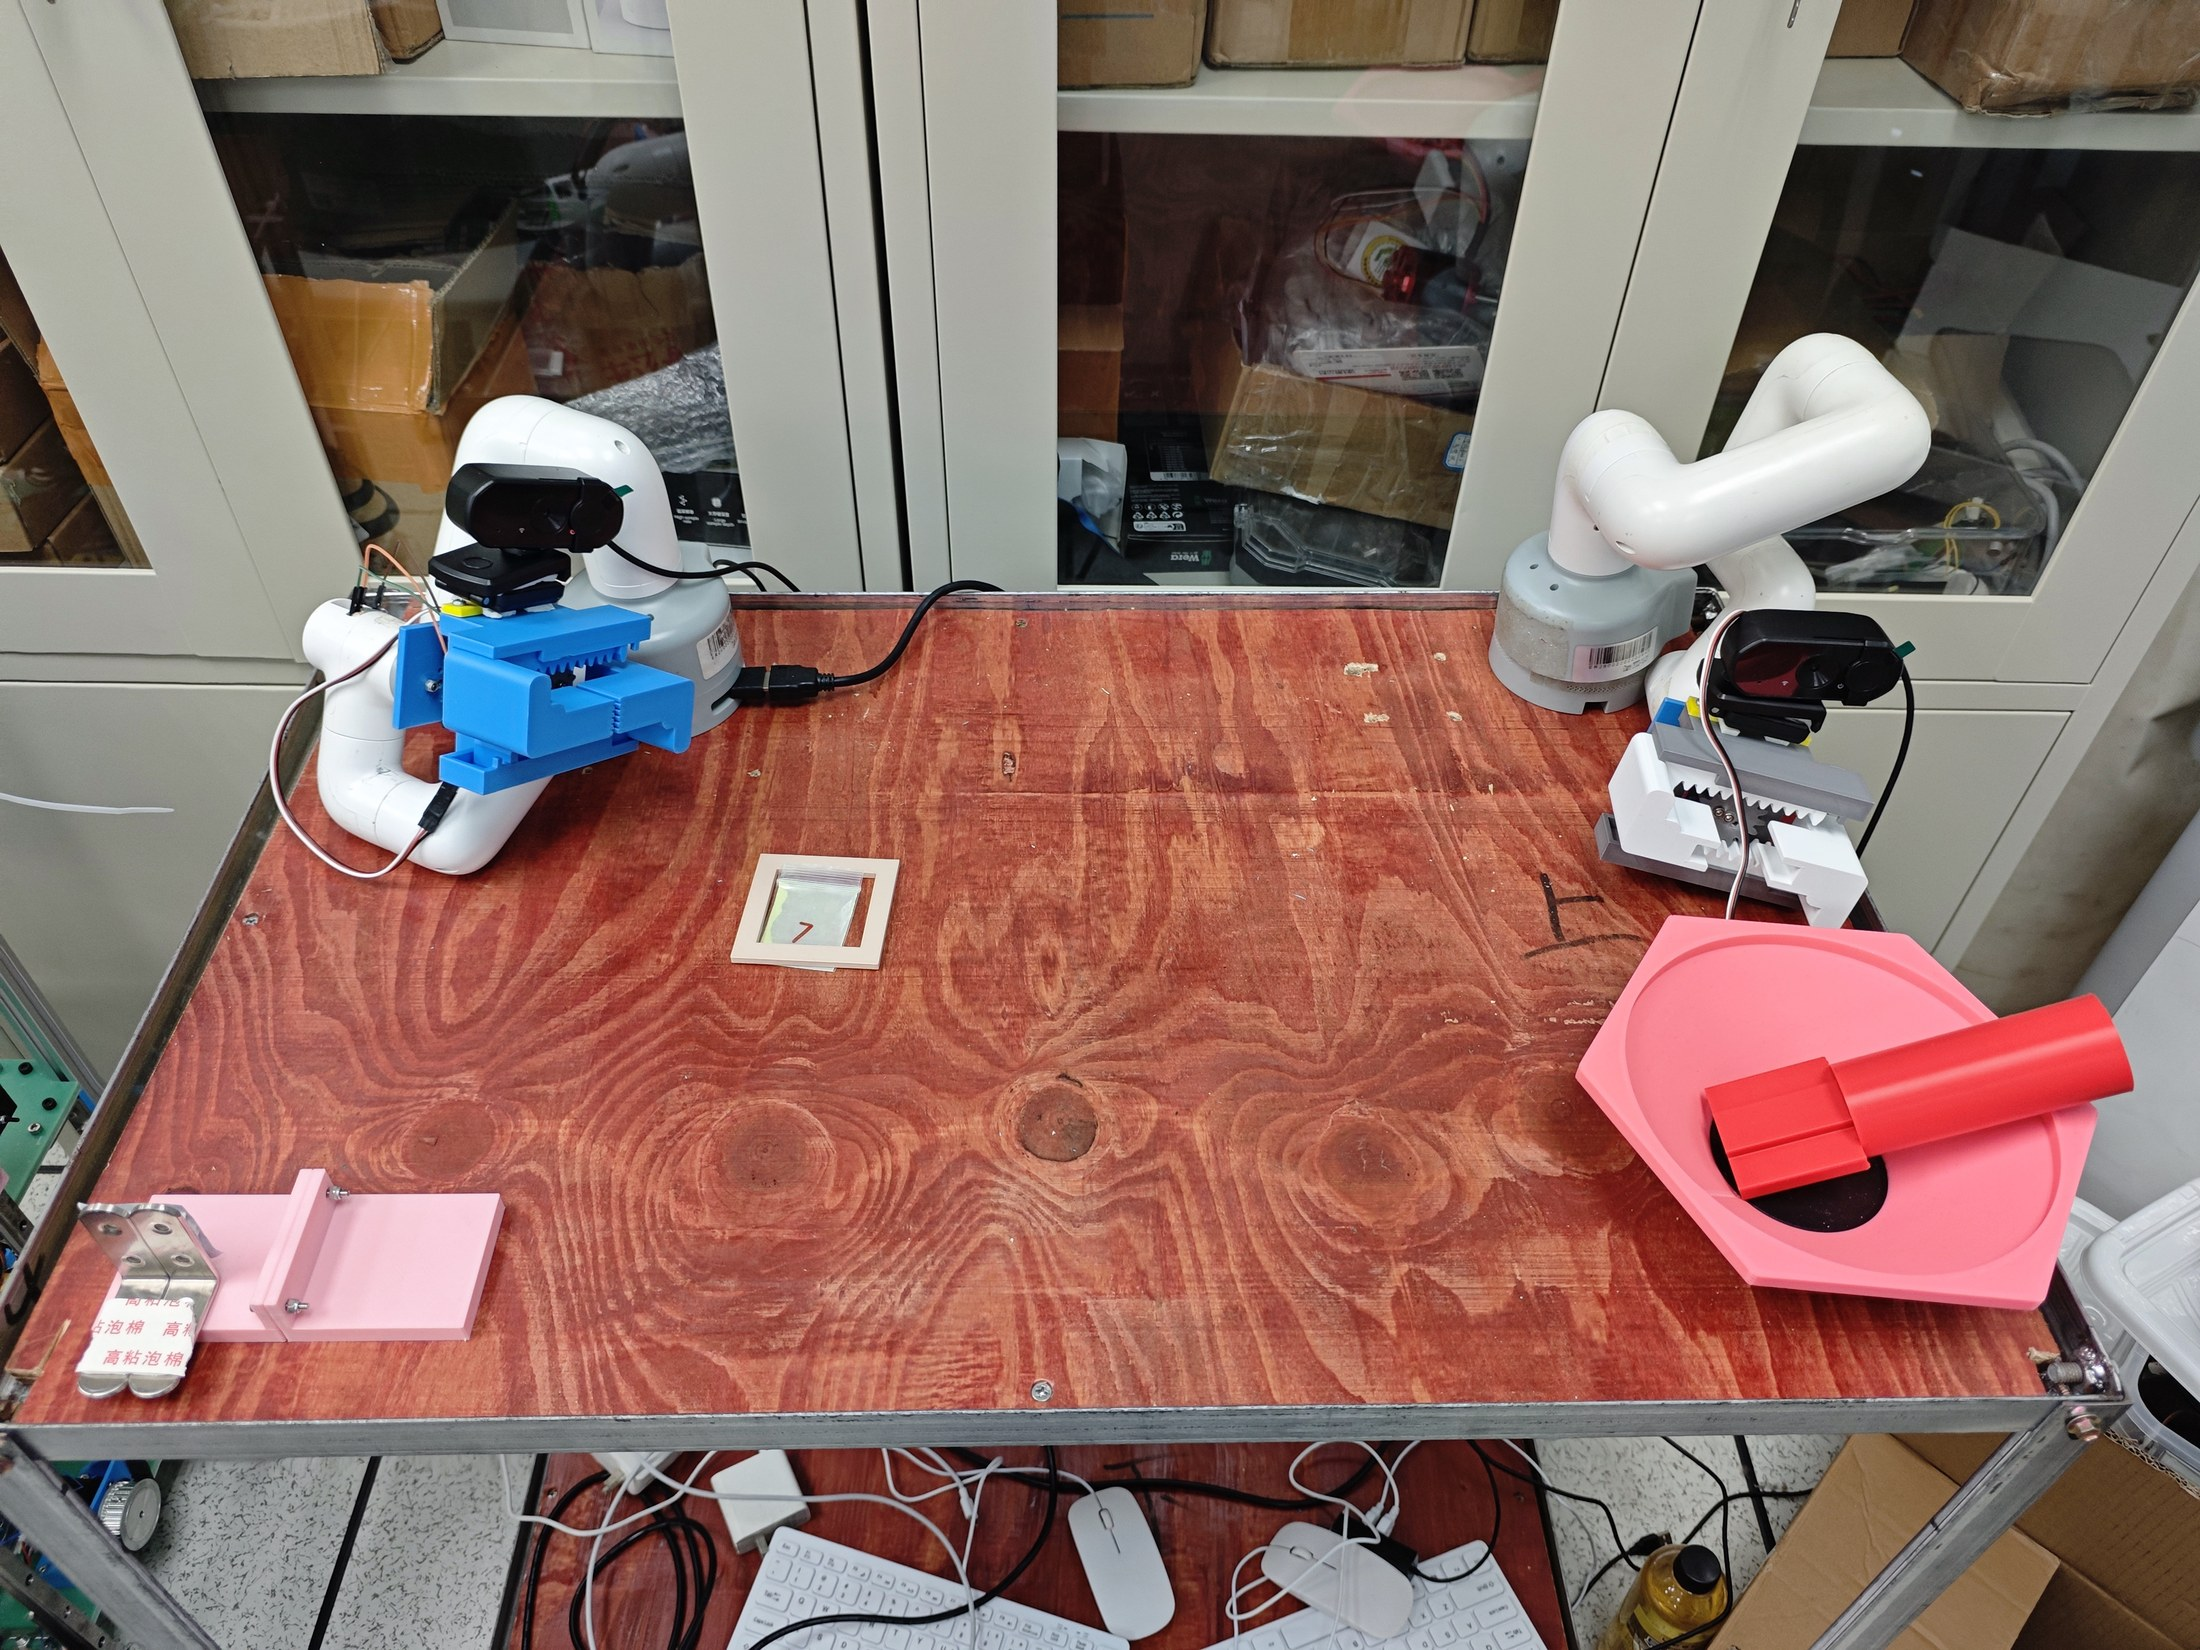
\includegraphics[width=\linewidth]{fig_actual_mech_workstation.jpg}
    \caption{双 myCobot 固定工位、视觉标记、夹爪与转运区域。}
  \end{subfigure}
  \caption{机械成果实物照片。车载端负责移动感知与末端执行，固定工位负责粉末袋识别、夹取和落袋。}
  \label{fig:actual_mechanical_results}
\end{figure}

\subsubsection*{3.2.2 电路成果}
\phantomsection
\addcontentsline{toc}{subsubsection}{3.2.2 电路成果}

电路与电气集成已经完成三层部署：顶层集成 LD14、云台/摄像头、显示与外设接口；中层布置升降、转运、视觉辅助和本地交互组件；底层集中放置 STM32F407、继电器/驱动板、电源模块、Astra 深度相机和电池。F407 负责舵机、电推杆、电磁铁和步进电机的动作时序，RDK X5 负责上层感知、规划、状态判断和安全门控。当前电磁铁与升降台按安全降级流程演示，后续加入顶部/底部限位、ALM 输入和驱动隔离后可接入完整自主闭环。

\begin{figure}[H]
  \centering
  \begin{subfigure}{0.32\linewidth}
    \centering
    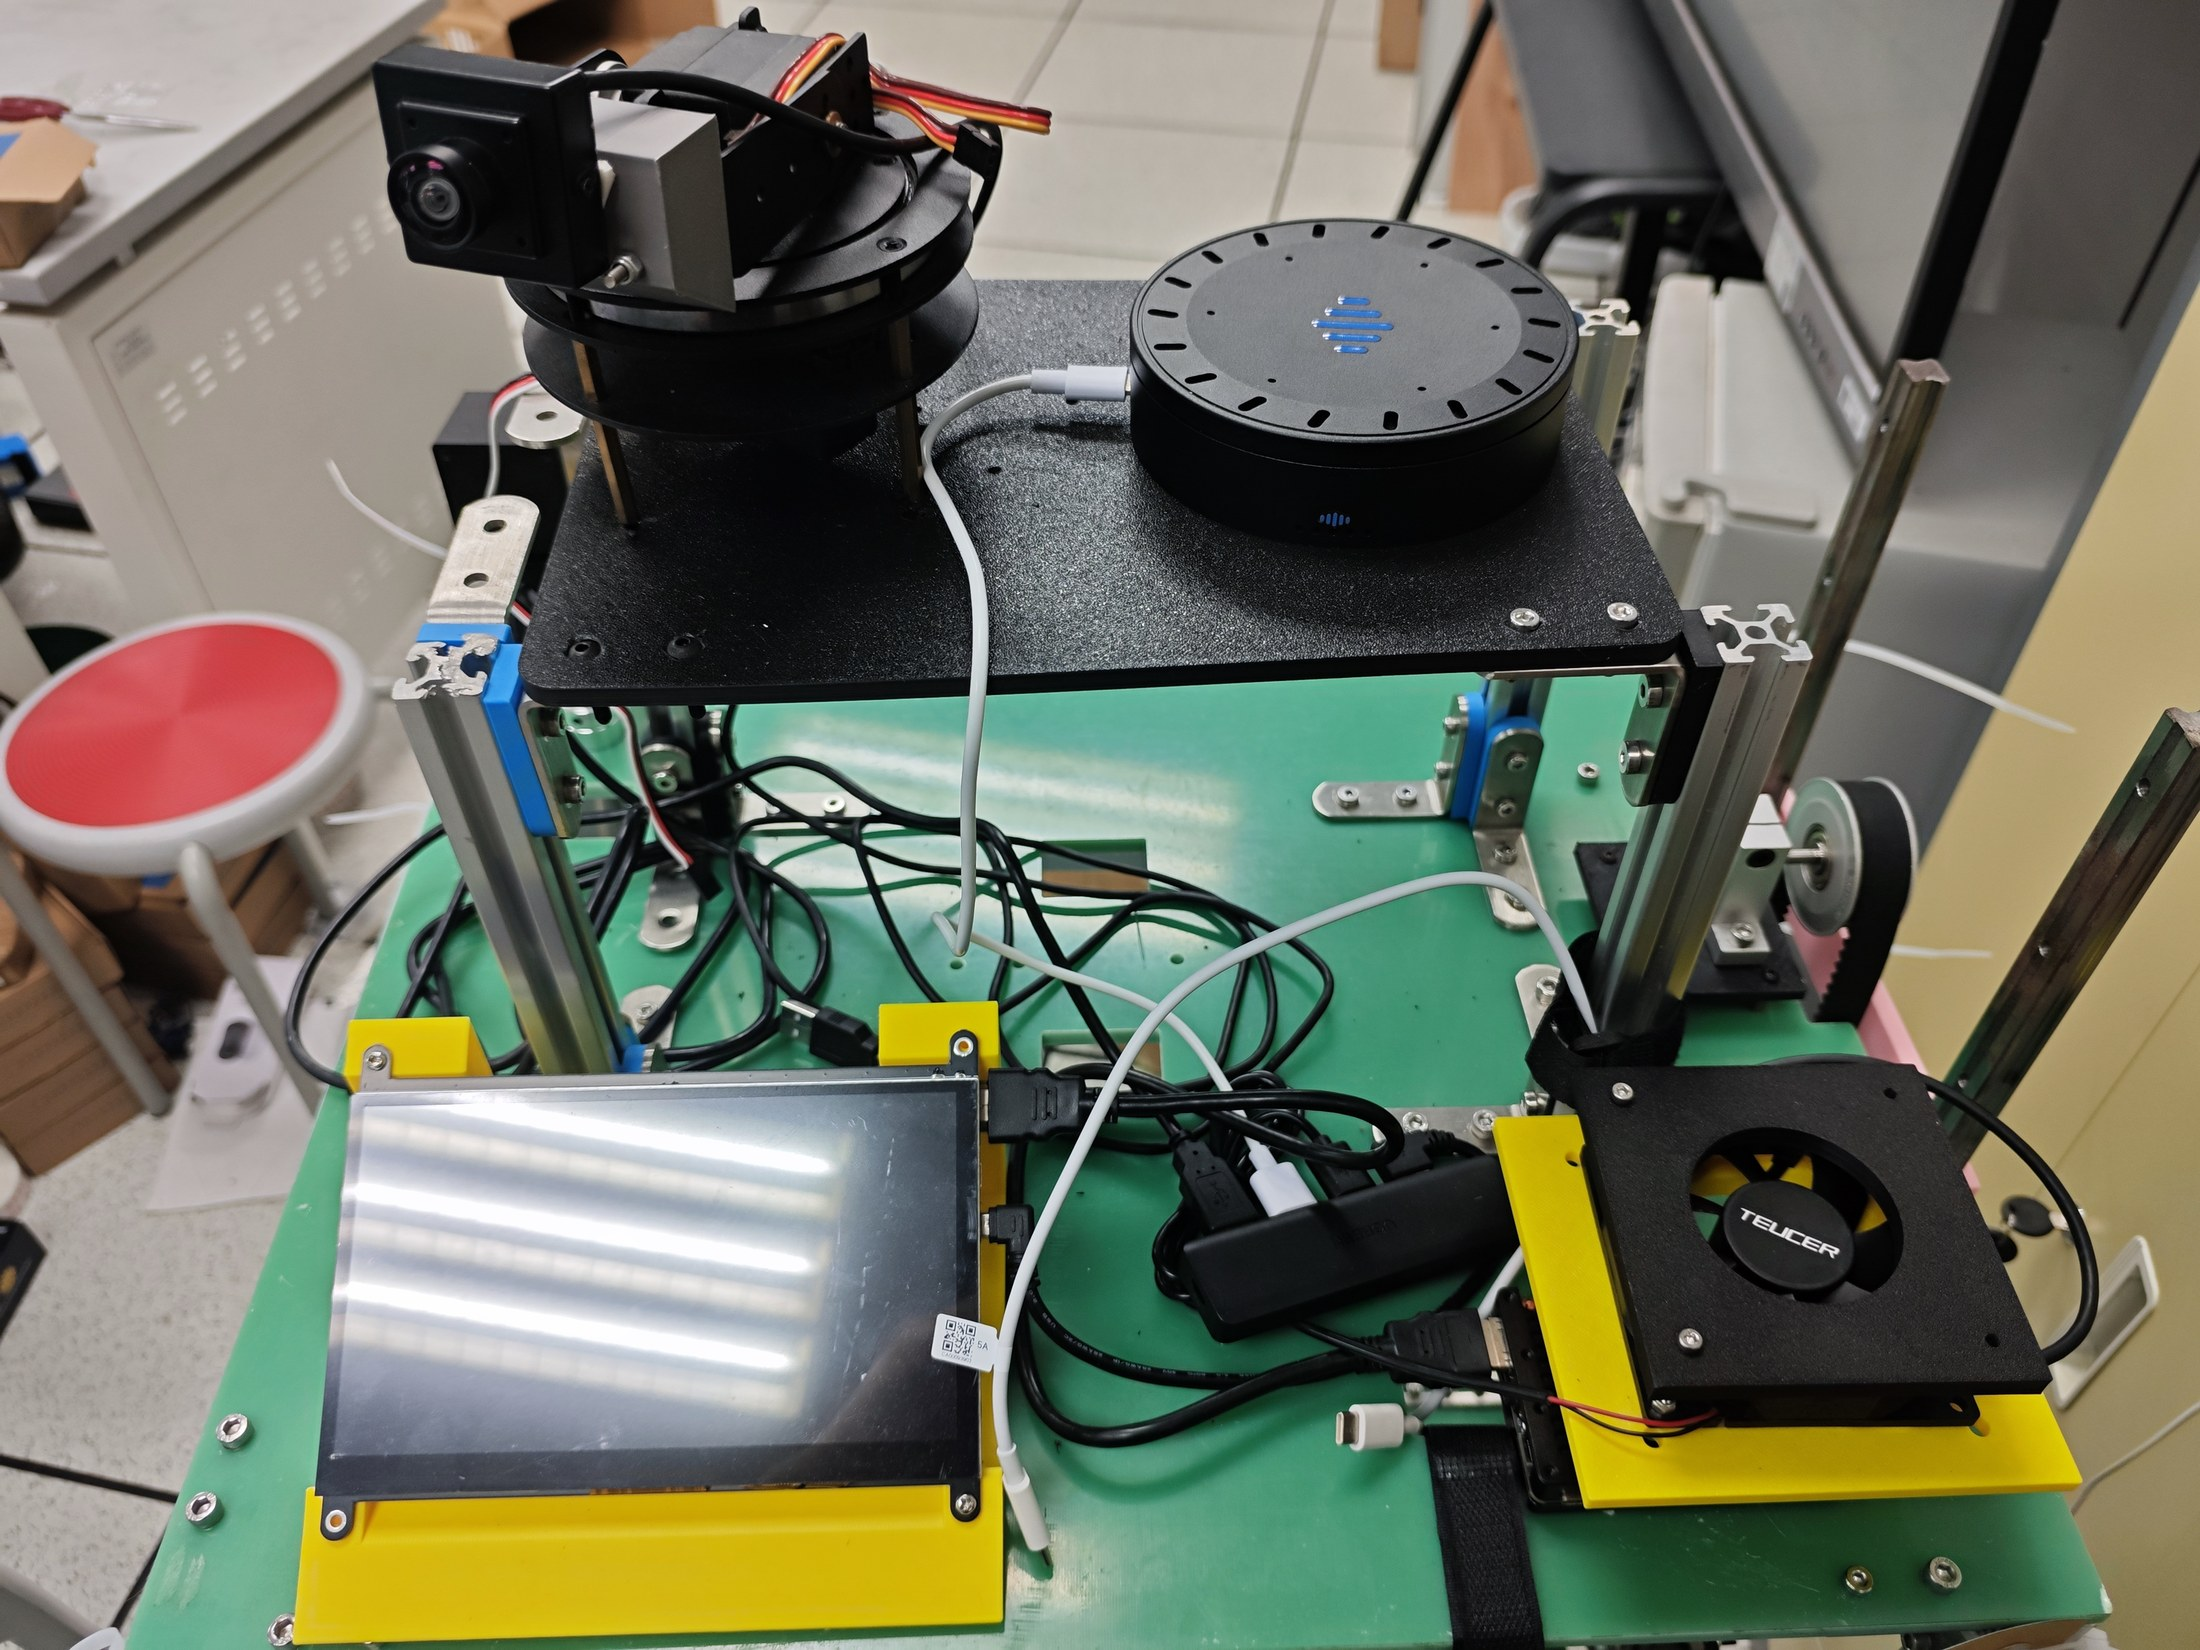
\includegraphics[width=\linewidth]{fig_actual_circuit_top.jpg}
    \caption{顶层传感器、云台、显示与线束。}
  \end{subfigure}
  \hfill
  \begin{subfigure}{0.32\linewidth}
    \centering
    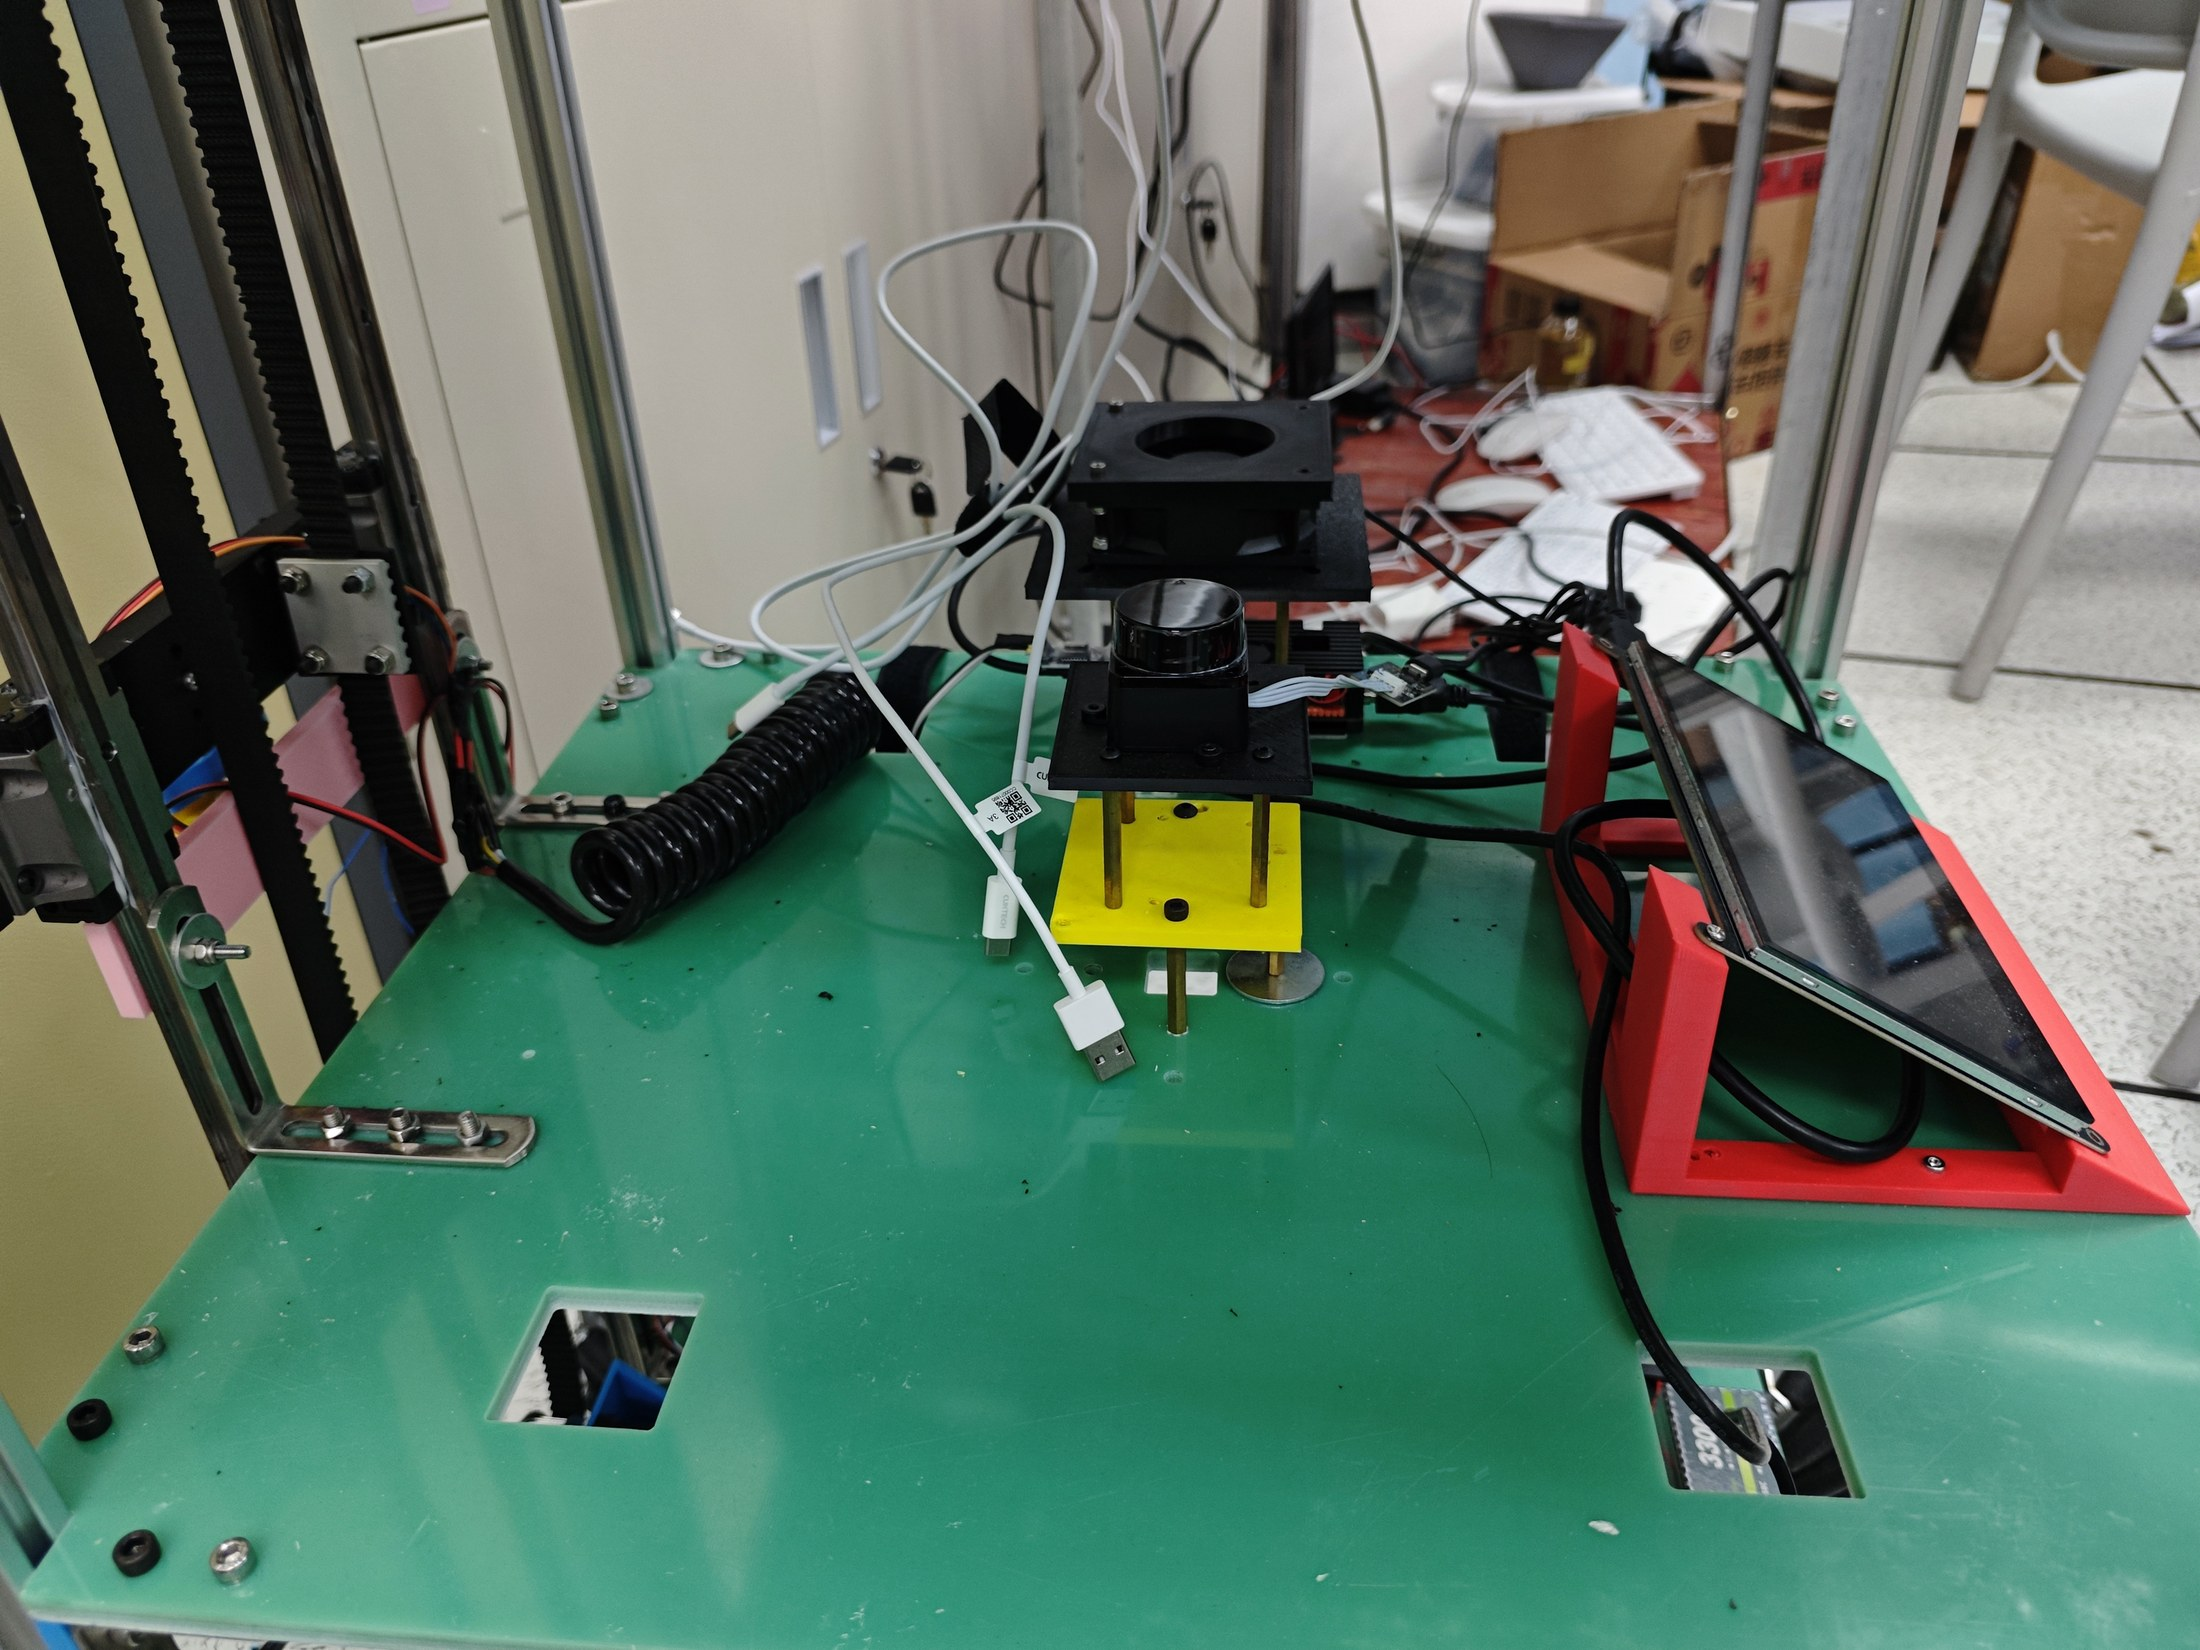
\includegraphics[width=\linewidth]{fig_actual_circuit_mid.jpg}
    \caption{中层升降/转运执行与本地交互。}
  \end{subfigure}
  \hfill
  \begin{subfigure}{0.32\linewidth}
    \centering
    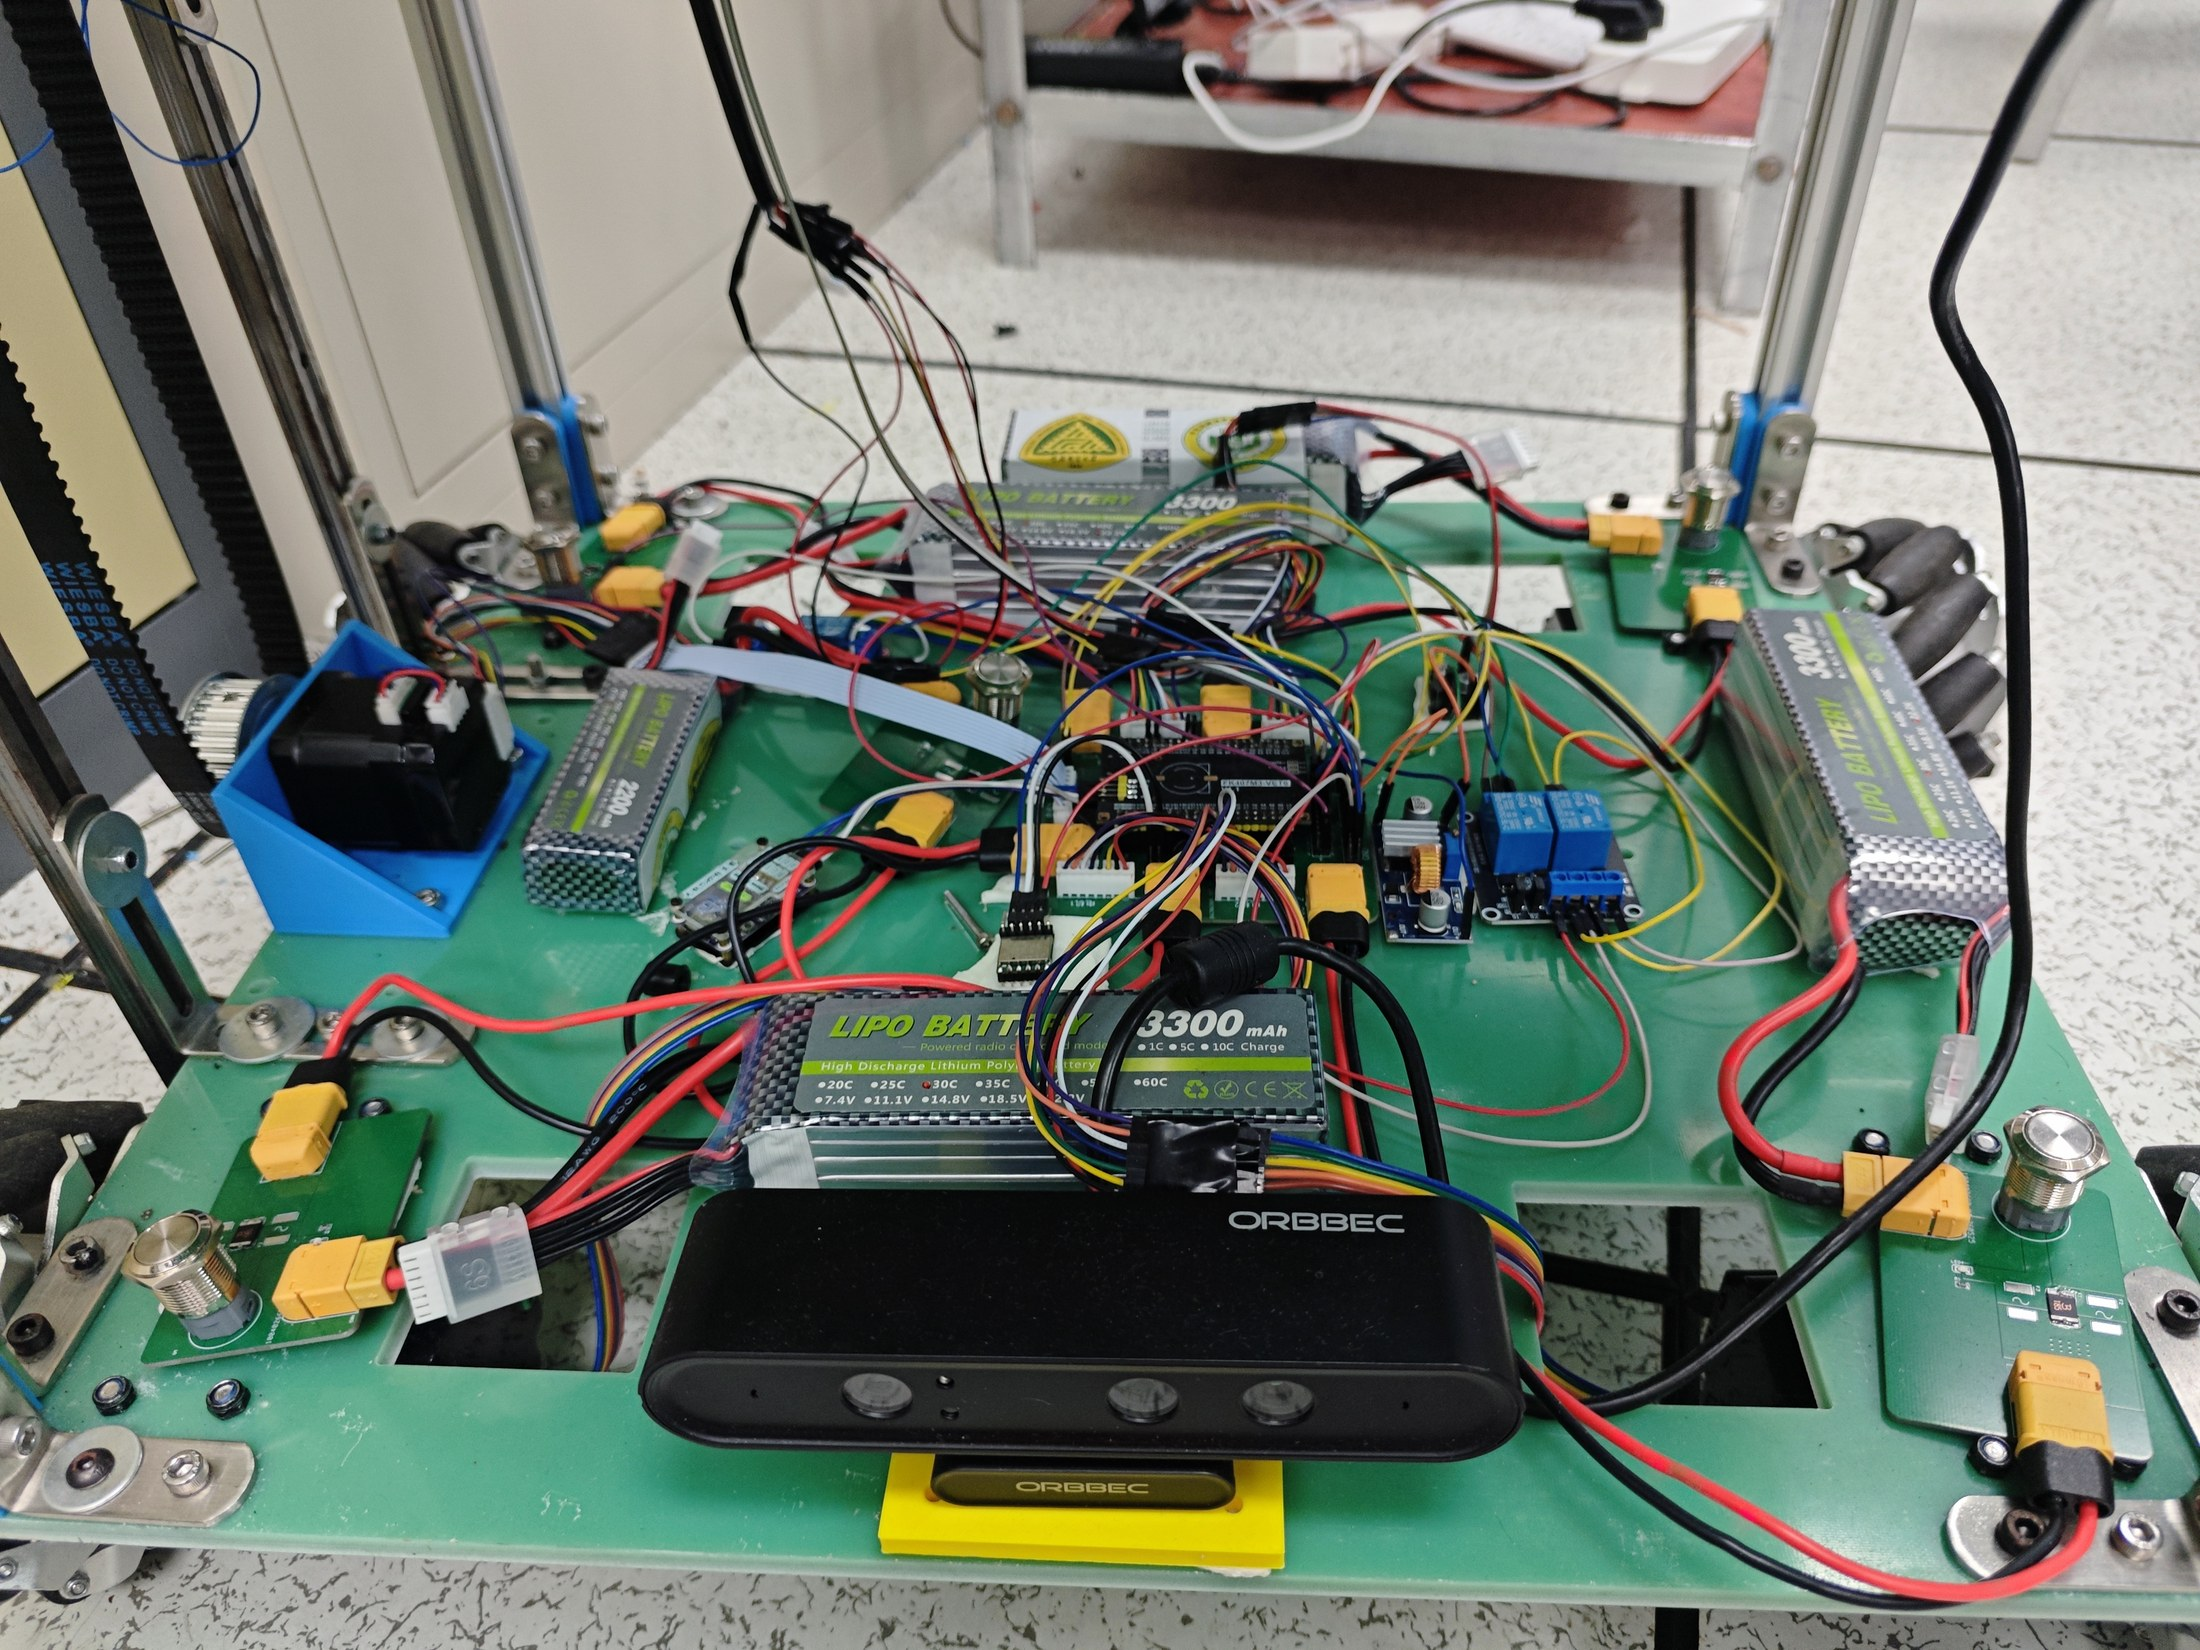
\includegraphics[width=\linewidth]{fig_actual_circuit_base.jpg}
    \caption{底层 F407、电源、继电器、深度相机与驱动。}
  \end{subfigure}
  \caption{电路成果实物照片。系统将 RDK X5 高层决策、STM32F407 底层时序和多传感器输入集成到同一车载平台。}
  \label{fig:actual_circuit_results}
\end{figure}

\subsubsection*{3.2.3 软件成果}
\phantomsection
\addcontentsline{toc}{subsubsection}{3.2.3 软件成果}

软件成果包括 AI 脑材料预测平台、具身脑 Lab-FSD 世界模型、公网展示站和证据链平台。AI 脑侧接入视觉线、XRD 数值线、光谱视觉线和光谱数值线，完成配方预筛、物相/光谱解释、本地模型推理与失败回流；具身脑侧运行 SLAM、LD14、Astra 深度相机和 Lab-FSD shadow planner，输出 BEV occupancy、候选轨迹、风险等级和安全门控结果。公网展示站用于统一展示系统状态、模型能力、全球对标、FSD 世界模型、设备机群和可追溯资产。

\begin{figure}[H]
  \centering
  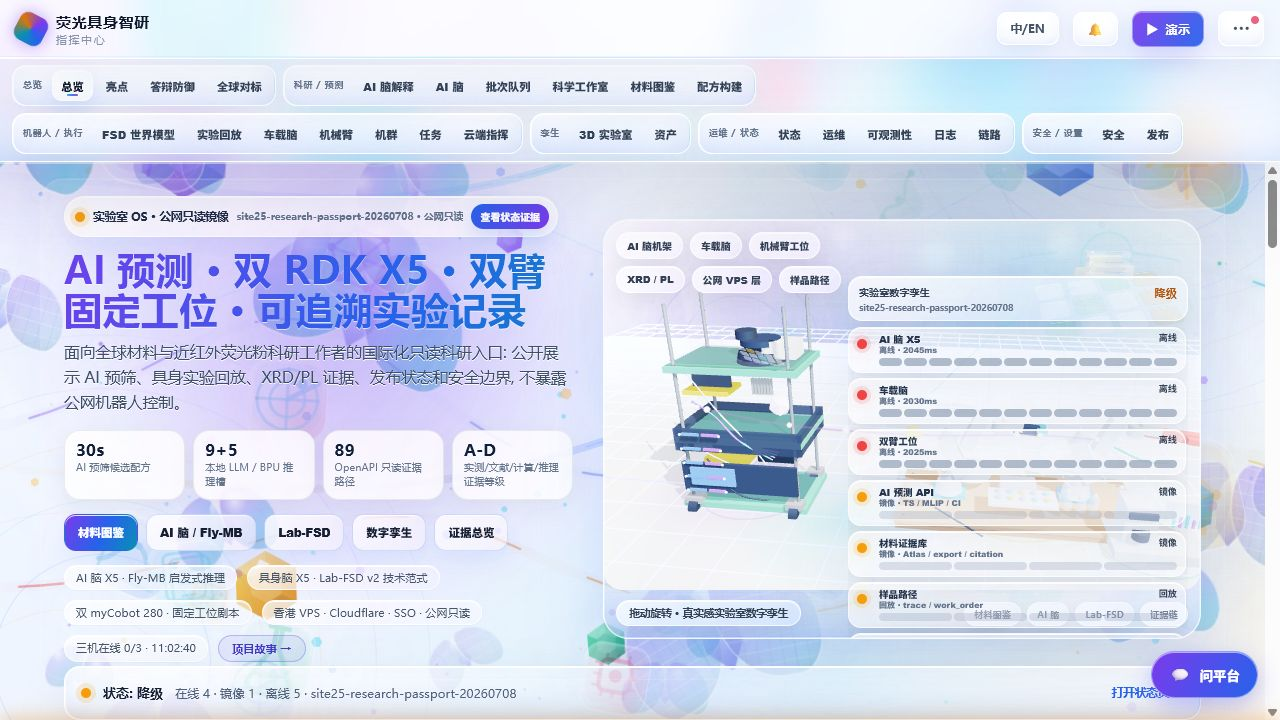
\includegraphics[width=0.98\linewidth]{fig_actual_software_home_20260709.png}
  \caption{软件成果界面：公网展示站总览页，集中显示双 RDK X5、双臂工位、AI 预测 API、材料证据库和状态孪生。}
  \label{fig:actual_software_home}
\end{figure}

\begin{figure}[H]
  \centering
  \begin{subfigure}{0.49\linewidth}
    \centering
    
\includegraphics[width=\linewidth]{fig_actual_software_ai_brain_20260709.png}
    \caption{AI 脑解释系统与 Fly-MB 材料判决界面。}
  \end{subfigure}
  \hfill
  \begin{subfigure}{0.49\linewidth}
    \centering
    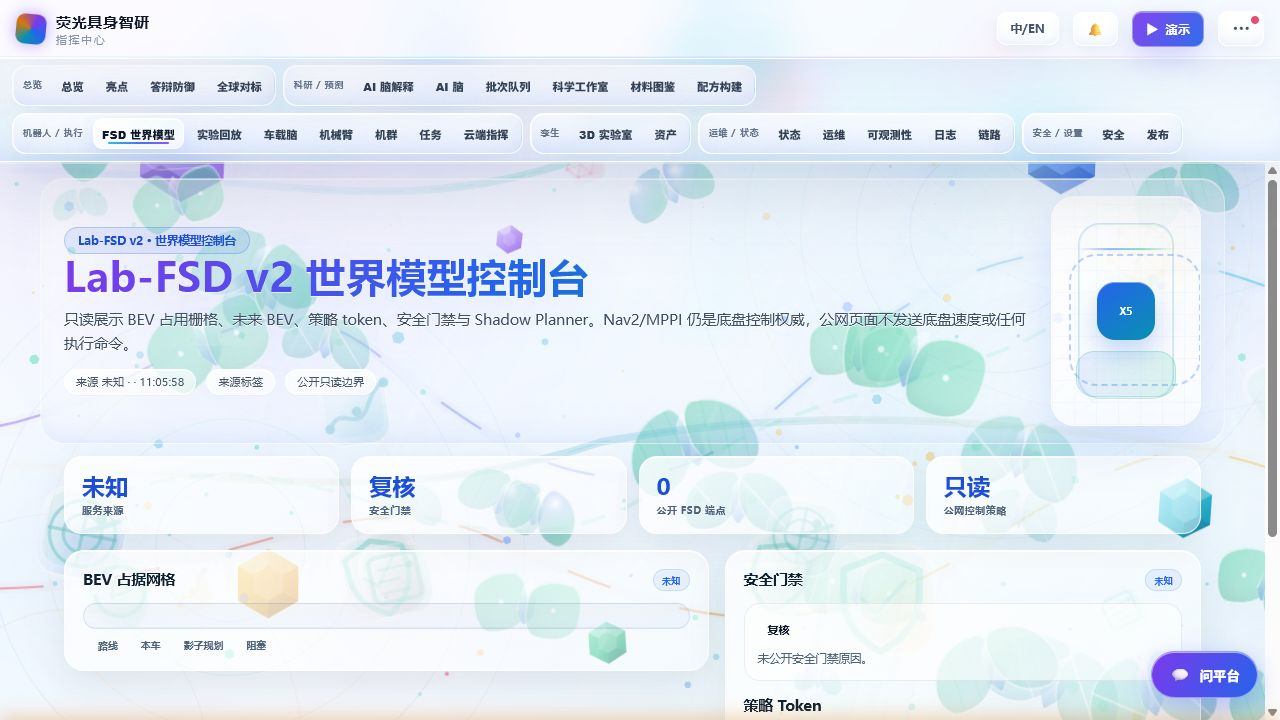
\includegraphics[width=\linewidth]{fig_actual_software_labfsd_20260709.png}
    \caption{Lab-FSD v2 世界模型与安全门禁界面。}
  \end{subfigure}
  \caption{软件成果界面：AI 脑负责科研推理和材料判决，具身脑负责实验室世界模型与 shadow planning。}
  \label{fig:actual_software_brain_fsd}
\end{figure}

\subsection*{3.3 特性成果}
\phantomsection
\addcontentsline{toc}{subsection}{3.3 特性成果}

特性成果按功能完成度、量化指标和现场可展示证据列出。表~\ref{tab:feature_results} 中的“已实测”表示已在真实硬件或本地服务链路中跑通；“shadow/安全降级”表示感知、规划或动作时序在线运行，但出于初赛拍摄和硬件保护要求，不直接接管危险执行环节。

\begin{table}[H]
\centering
\caption{功能完成情况与性能参数汇总。}
\label{tab:feature_results}
\begin{tabular}{p{3.2cm}p{4.3cm}p{6.4cm}}
\toprule
模块 & 完成状态 & 关键参数与证据 \\
\midrule
双 RDK X5 异构架构 & 已实测 & AI 脑负责材料预测、XRD/PL 分析、本地大模型推理；具身脑负责 LiDAR、深度、里程计、SLAM 与 Lab-FSD shadow planning。 \\
AI 脑材料预测 & 已实测 & 五服务线接入；同步预测通常小于 5 s；本地 CPU LLM、BPU slot、小模型分类器和云端 R1 构成多级判决链路。 \\
BPU 本地推理 & 已实测 & 轻量 MLP 分类器小于 2 ms；YOLO 谱图检测约 110 ms/frame；Qwen2-0.5B BPU slot forward 约 553 ms。 \\
XRD/PL 表征分析 & 已实测 & XRD 45D/190D 数值特征、PL 80D 光谱特征、视觉检测和大模型解释可由平台统一调用并回流实验记录。 \\
SLAM 与移动感知 & 已跑通 & LD14 提供二维障碍结构，Astra 补充近距离深度，现场 SLAM 占据栅格已生成，用于导航边界和安全门控初始化。 \\
Lab-FSD shadow planner & 在线运行 & 输出 BEV occupancy、future BEV、policy token、候选轨迹、风险等级与 safety gate；初赛不直接接管底盘。 \\
机械臂取袋闭环 & 已实测 & arm01 末端相机识别 AprilTag 工位标记，AI 脑返回 \texttt{station\_ok=true} 后执行固定点夹取、转运与落袋。 \\
STM32F407 末端执行 & 安全降级已跑通 & 舵机、电推杆、电磁铁和升降机构动作时序已验证；瓶子吸附、保持、释放流程已用于初赛演示。 \\
公网展示与证据链 & 已部署 & 展示站包含总览、亮点、答辩防御、全球对标、FSD 世界模型、机群和资产页；OpenAPI 只读证据路径 89 条。 \\
\bottomrule
\end{tabular}
\end{table}

\begin{figure}[H]
  \centering
  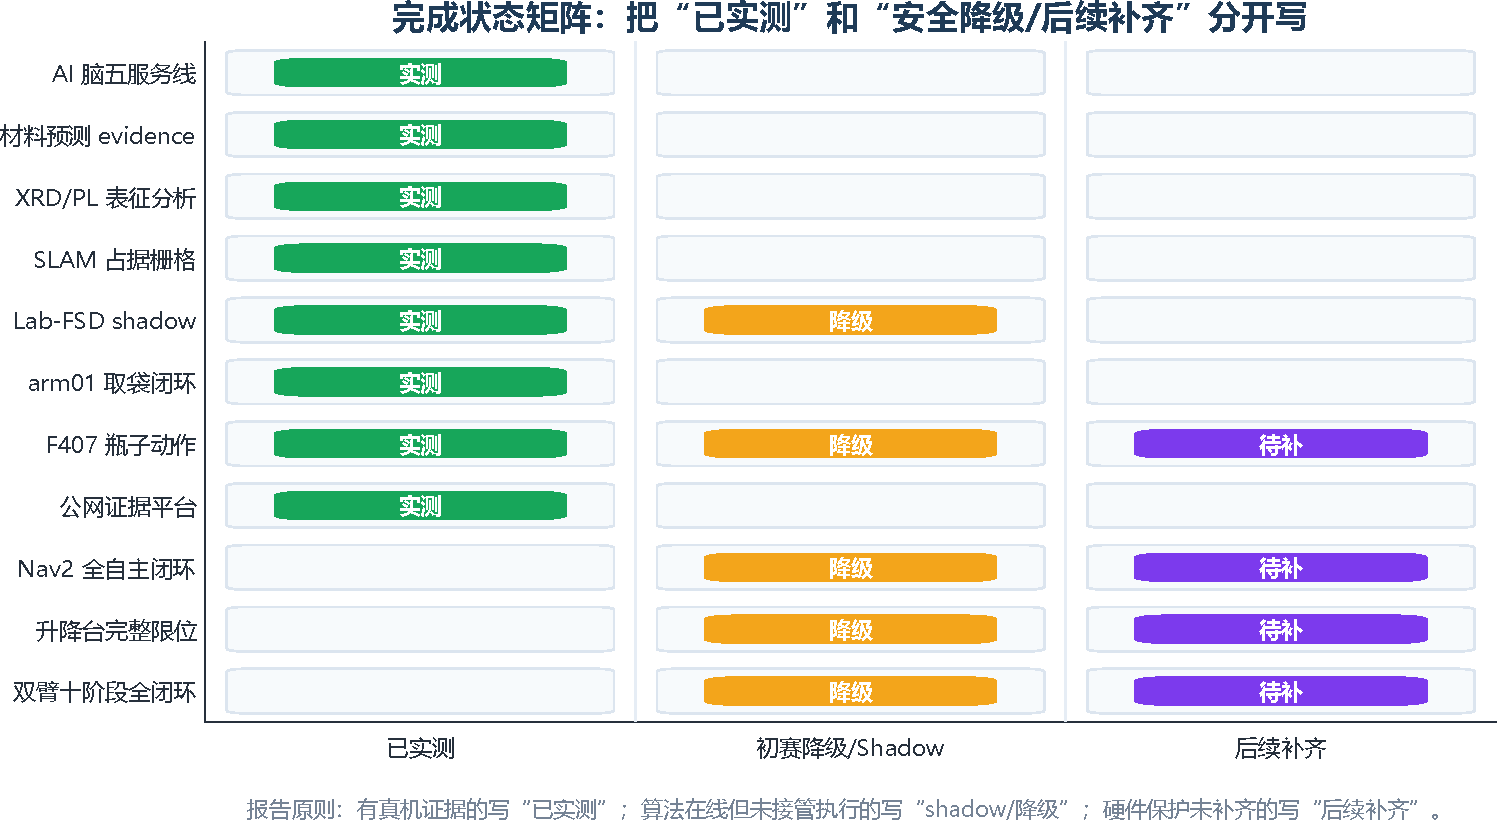
\includegraphics[width=0.95\linewidth]{fig_xrd_completion_matrix.pdf}
  \caption{完成状态矩阵：区分已实测、shadow/安全降级和后续升级项，防止把观察模式写成完全自主闭环。}
  \label{fig:xrd_completion}
\end{figure}

\begin{figure}[H]
  \centering
  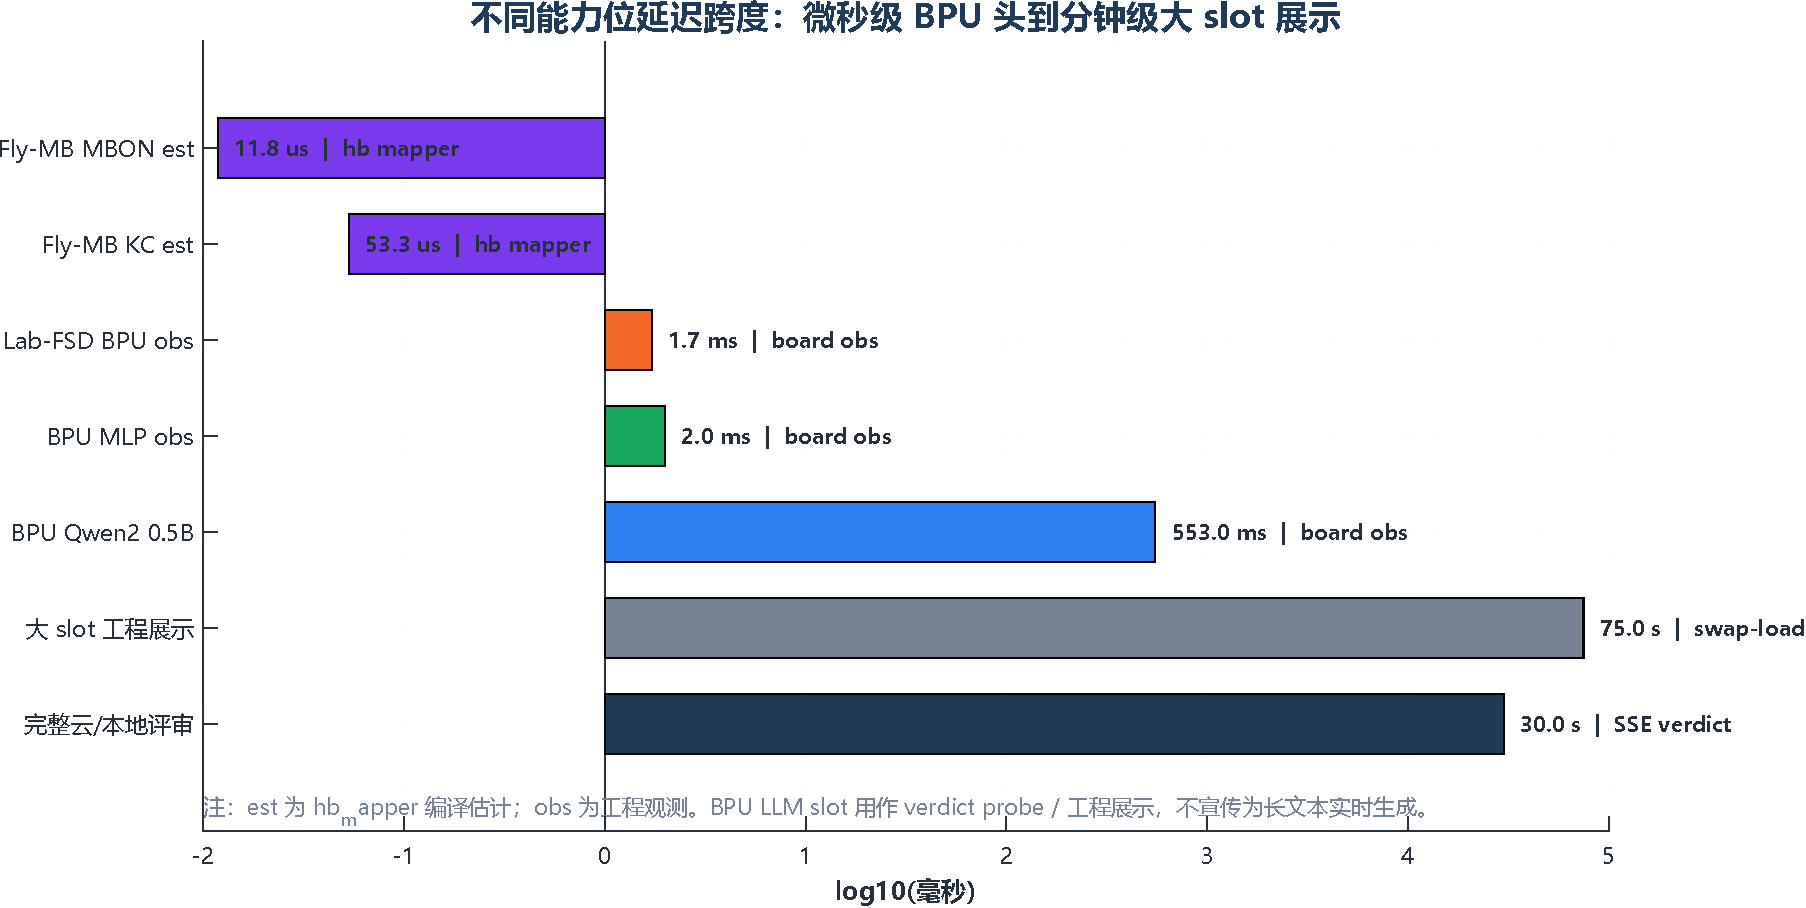
\includegraphics[width=0.95\linewidth]{fig_xrd_latency.pdf}
  \caption{关键链路性能参数：材料预测、BPU/CPU 推理、机械臂视觉确认、SLAM 与公网平台接口的延迟量级。}
  \label{fig:xrd_latency_validation}
\end{figure}

综合来看，项目已实现“材料问题输入 - AI 预测与表征解释 - 具身感知与安全规划 - 机械臂/末端执行 - 实验记录与公开证据”的端到端工程样机。当前演示采用安全员接管底盘和局部执行安全降级，核心传感、规划、材料判决、机械臂取放、F407 动作时序和证据平台均在线运行，具备继续接入限位、Nav2 目标点和更多实验回流数据的基础。

\section{提交材料与公开边界说明}

\subsection{提交材料映射}
初赛提交材料包括作品视频、作品设计报告和重要代码压缩包。根据提交要求，视频控制在 3 分钟以内，报告 PDF 控制在 50 MB 以内，重要代码压缩包控制在 100 MB 以内。项目复杂度远高于单一演示，因此报告采用高密度图表和分章节工程说明，视频则以倍速和多窗口方式展示关键证据。
\begin{figure}[H]
  \centering
  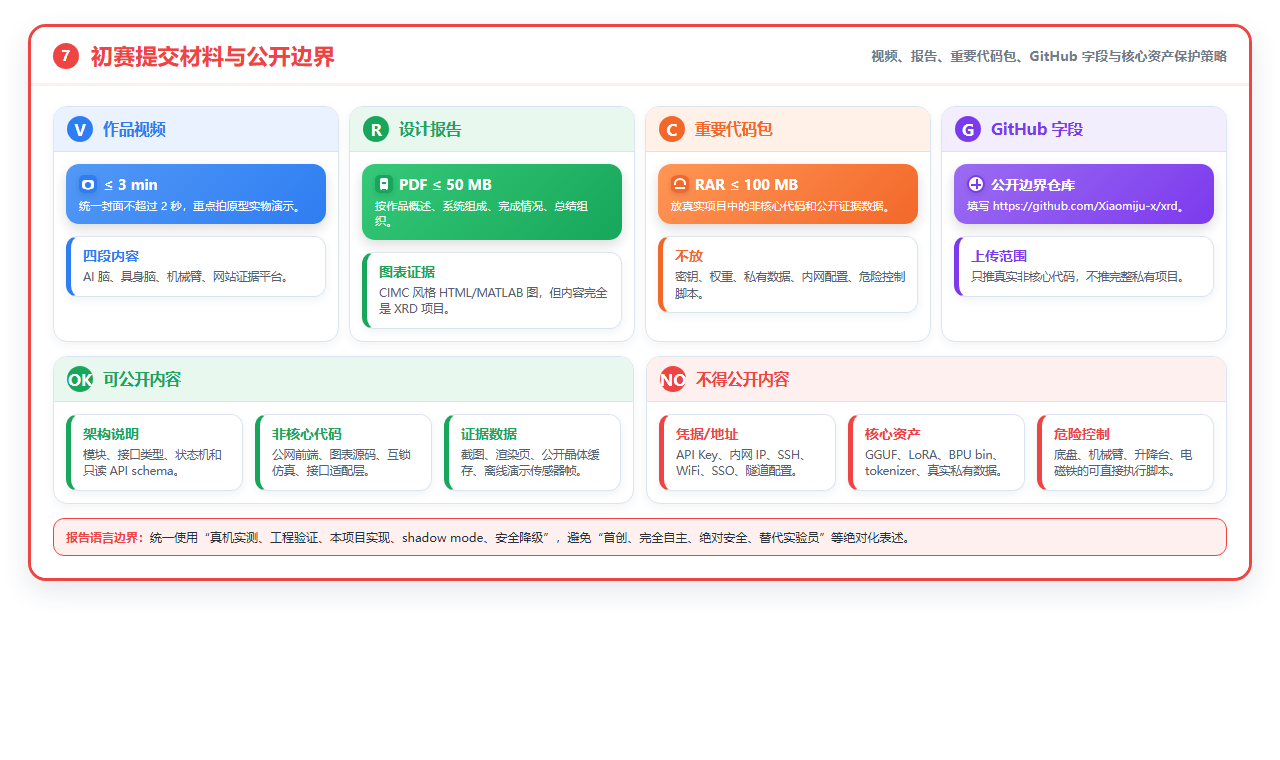
\includegraphics[width=\linewidth]{fig_xrd_submission_boundary_html.png}
  \caption{初赛提交材料与公开边界。}
  \label{fig:xrd_submission}
\end{figure}

\subsection{重要代码包边界}
重要代码包采用“真实项目代码、非核心公开边界”的原则：上传可审查的公网展示站静态前端、报告图表生成脚本、工位碰撞互锁与仿真逻辑、接口 schema、公开演示适配层、公开证据截图、报告渲染页、晶体结构公开缓存和离线演示传感器帧。代码包保留接近提交上限的工程证据体量，同时不公开以下内容：
\begin{itemize}
  \item API Key、账号、Cookie、SSH、WiFi、隧道配置、内网地址和任何可登录凭据；
  \item GGUF、LoRA、BPU bin、tokenizer、tensor 包等模型权重；
  \item 未发表实测数据、原始谱图、failure patterns、私有实验记录和完整训练数据；
  \item 核心预测引擎、可直接复现实验室策略的私有规则库和部署脚本；
  \item 可直接控制底盘、机械臂、升降台、电磁铁或舵机的危险执行脚本；
  \item 任何学校、个人、导师或账号身份信息。
\end{itemize}

\subsection{GitHub 字段}
GitHub 字段填写项目公开边界仓库：
\begin{center}
  \url{https://github.com/Xiaomiju-x/xrd}
\end{center}
该仓库用于提交审查和技术展示，内容限定为真实项目的非核心代码、文档、接口 schema 和可离线查看的前端资产；不上传完整工程、模型权重、私有数据、部署凭据和核心材料预测引擎。报告、视频与仓库对外口径保持一致：强调真机实测、工程验证、shadow mode、安全降级和可追溯证据链。

\begin{warnbox}
报告、视频和公开代码包统一避免绝对化、宣传式或过度承诺措辞，统一使用“真机实测”“工程验证”“本项目实现”“shadow mode”“安全降级”等可防守表述。
\end{warnbox}

\section{第四部分 总结}

\subsection{主要结论}
本作品完成了一套面向材料研发场景的双 RDK X5 嵌入式智能系统。它的复杂度来自跨域耦合：材料科学模型需要和 BPU/CPU 本地推理结合，AI 脑需要和 XRD/PL 表征线结合，具身脑需要和 LiDAR、深度、SLAM、Lab-FSD shadow 结合，机械臂工位和 F407 需要在安全边界内执行真实动作，公网平台需要把这些证据组织成评审可理解的页面。

相比只展示某个模型、某个网页或某台机械臂，本作品更接近一个实验室级嵌入式系统。它已经跑通的内容包括材料预测、四条表征线、SLAM 建图、Lab-FSD shadow、arm01 视觉门控取袋、F407 末端动作和公网证据平台；尚未完全闭环的内容也被明确标注为 shadow、降级或后续补齐。

\subsection{可扩展方向}
后续可扩展方向包括：
\begin{itemize}
  \item 补齐升降台限位和电磁铁驱动隔离，使 F407 工位具备更完整的无人值守安全保护；
  \item 优化 SLAM 地图质量，接入 Nav2 目标点和受限场景下的导航闭环；
  \item 扩展双臂十阶段剧本，将承碗、研磨、灌装、取烧结样和 XRD/PL 回填逐步真机化；
  \item 增加更多真实实验回流数据，改进 failure library、Fly-MB 记忆和材料预测置信度；
  \item 将公网展示站继续收敛为 Research Passport 和 Evidence Bundle，使复杂工程可复核、可答辩、可复现。
\end{itemize}

\subsection{心得体会}
项目推进中最重要的经验是：复杂嵌入式系统不能只追求“看起来全自动”，而要把每一层的真实边界写清楚。AI 预测不能替代烧制和表征，Lab-FSD 不能越过安全门直接接管底盘，F407 末端执行不能在限位未补齐时写成无人值守全闭环，公网平台不能开放危险控制。正是这些边界让系统在初赛阶段既能展示工程量，也能保持可信和可继续迭代。

\section{第五部分 参考文献}
\begin{enumerate}
  \item Horizon Robotics. RDK X5 development board and Bayes-e BPU documentation.
  \item Open Robotics. ROS 2 documentation.
  \item Nav2 Project. Navigation2 documentation and MPPI controller documentation.
  \item A. Vaswani et al. Attention Is All You Need. NeurIPS, 2017.
  \item Z. Li et al. BEVFormer: Learning Bird's-Eye-View Representation from Multi-Camera Images. ECCV, 2022.
  \item Y. Hu et al. Planning-oriented Autonomous Driving. CVPR, 2023.
  \item B. Jiang et al. VAD: Vectorized Scene Representation for Efficient Autonomous Driving. ICCV, 2023.
  \item X. Zheng et al. OccWorld: Learning a 3D Occupancy World Model for Autonomous Driving. 2023.
  \item G. Blasse, B. C. Grabmaier. Luminescent Materials. Springer, 1994.
  \item V. Rajendran et al. Recent progress on broadband near-infrared phosphors-converted LEDs. Optical Materials: X, 2019.
  \item R. D. Shannon. Revised effective ionic radii and systematic studies of interatomic distances in halides and chalcogenides. Acta Crystallographica A, 1976.
  \item A. Jain et al. The Materials Project: A materials genome approach to accelerating materials innovation. APL Materials, 2013.
\end{enumerate}


\end{document}
